\documentclass [german,a4paper,11pt,oneside,webreferences,glossary,indextop,listoflistings,todo]{INSOthesis}
% change encoding in the document
%\inputencoding{utf8} % default
%\inputencoding{latin1} % for windows

\thesistitle{Model-based Testing auf Basis von Fachmodellen in großen agilen Entwicklungsumgebungen}
%\thesisshorttitle{Shorttitle of the Thesis}
%\thesissubtitle{Optional Subtitle} % optional
\thesisdate{\today}

% all titles and designations have to be gender-related!
\thesistype{Diplomarbeit}{Master's Thesis}
%\thesisdegree{Diplom-Ingenieurin}{Diplom-Ingenieurin}
\thesiscurriculum{Software Engineering and Internet Computing}{Software Engineering and Internet Computing} % your study
\thesisauthor{Ramón López Narváez} % your name
\thesisauthoraddress{Konradgasse 1/30, 1020 Wien} % your address
\thesismatrikelno{1328066} % your registration number

% advisor
%\thesisauthorpreamble {Verfasser}
%\thesisadvisorpreamble {Betreuung}
%\thesisadvisorone {Thomas Grechenig}
\thesisadvisortwo {Boris Wrubel}
%\thesisadvisorthree {Vorname Nachname}

% Bibliographie file
\bibliography{bibliography/references}

\hypersetup{
  %colorlinks=false % enable and disable frames arround links
}

%%%%%%%%%%%%%%%%%%%%%%%%%%%%%%%%%%%%%%%%%%%%%
%
% Can be used to add additional informations
%
%%%%%%%%%%%%%%%%%%%%%%%%%%%%%%%%%%%%%%%%%%%%%
% \AfterTitlePages{}
% \AfterDeclaration{}
% \AfterAcknowledgements{}
% \AfterAbstract{}
% \AfterListOfFigures{}
% \AfterListOfTables{}
% \AfterAbbreviations{}
% \AfterBibliography{}

\renewcommand\afterchapternum{\hspace{1em}}
\begin{document}

\maketitle

%%%%%%%%%%%%%%%%%%%%%%%%%%%%%%%%%%%%%%%%%
%%%   CONTENTS    %%%%%%%%%%%%%%%%%%%%%%%
%%%%%%%%%%%%%%%%%%%%%%%%%%%%%%%%%%%%%%%%%

%%%%%%%%%%%%%%%%%%%%%%%%%%%%%%%%%%%%%%%%%%%%%%%%%%%%%%%%%%%%%%%%%%%%%%%%
\chapter{Einleitung}
\label{sec:introduction}
%%%%%%%%%%%%%%%%%%%%%%%%%%%%%%%%%%%%%%%%%%%%%%%%%%%%%%%%%%%%%%%%%%%%%%%%

%=======================================================================
\section{Problemstellung}
%=======================================================================

Steigende Komplexität in modernen technischen Disziplinen, darunter auch die Softwareentwicklung, erfordern Methoden zur Qualitätssicherung. Systematisches Prüfen ist ein zentrales Mittel, um Qualität von Software über einen längeren Zeitraum hinweg sicherzustellen \cite{spillner_software_2014}. Automatisierte Softwaretests auf Integrations- und Systemebene haben sich als effizienter Kontrollmechanismus etabliert \cite{dustin_software_2000}, sind aber herausfordernd in ihrer Umsetzung, vor allem in agilen Entwicklungsumgebungen. Kurze Iterationen, kombiniert mit einer hohen Frequenz von Änderungen in der Software erfordern spezialisierte Methoden \cite{linz_testing_2014}. Allein die Wahl des richtigen Werkzeugs für automatisiertes Testen garantiert noch keine erfolgreiche Teststrategie. Ungeachtet der gewählten Teststrategie, kann das Warten von Testfällen einen erheblichen Ressourcenaufwand verursachen der über Erfolg und Misserfolg eines Softwareprojekts entscheiden kann \cite{dustin_software_2000}. Vor allem agile Teams arbeiten auf multifunktionaler Basis. Deshalb darf sich auch die Generierung und Wartung von Testfällen nicht nur den technischen Rollen erschließen \cite{linz_testing_2014}. Bei mehreren weitverbreiteten Technologien ergibt sich aber genau diese Problematik.\\
%%%
%%%Ein vielversprechender Ansatz ist Testen auf Basis von Modellen, sogenannten %%%modellbasiertes Testen. Beim modellbasierten Testen wird die zu testende Applikation als %%% Modell in abstrahierter Form dargestellt. Daraus werden Testfälle automatisch generiert.
%%%%

%=======================================================================
\section{Motivation}
%=======================================================================
Kommerzielle Softwareprojekte sind teuer in der Entwicklung und der Wartung. Sie müssen unter hohem Zeitdruck geplant, spezifiziert, implementiert und ausgeliefert werden. Außerdem sollen solche Systeme dann oft mehrere Jahre betreut und in ihrer Funktionalität erweitert werden. Softwaresysteme die sensible Daten verarbeiten (Finanzwesen, Gesundheitswesen etc.) sind davon abhängig sehr exakte Ergebnisse zu liefern. Strenges Prüfen dieser ist unumgänglich. Gleichzeitig verknappen solche Tätigkeiten den engen zeitlichen Rahmen solcher Projekte. Deshalb wird, unabhängig von der Branche, das automatisierte regressive Testen von Software thematisiert \cite{graham_experiences_2012}.\\
Für jede gängige Programmiersprache und Plattform gibt es mächtige Test \Glspl{Framework}, die das Verhalten eines Benutzers automatisiert emulieren. In die Entwicklung von Testfällen mittels dieser \Glspl{Framework} fließt eine beträchtliche Anzahl an Ressourcen (laut \citeauthor{pol_management_2002} durchschnittlich 30\% - 40\% des Projektbudgets \cite{pol_management_2002}). Weiterhin ungelöst ist aber die Frage, wie es möglich ist diese Technologien intelligent, vielleicht sogar lernend (siehe Kapitel \ref{sec:test_based_modelling} \nameref{sec:test_based_modelling}), in die Entwicklung zu integrieren. Bis dahin scheint es aber noch ein langer Weg zu sein, wie es das \textit{LearnLib}-Projekt von \citeauthor{steffen_introduction_2011} zeigt \cite{steffen_introduction_2011}.\\

In der Zwischenzeit sind Ansätze nötig, die die Erkenntnisse des automatisierten Softwaretests übernehmen und neuartige Methoden zur Qualitätserhöhung und Wartungsreduzierung einbringen. Einer dieser Ansätze ist das modellbasierte Testen, welches eine Schicht zwischen den logischen und technischen Teil eines Tests zieht. Es findet also eine Abstrahierung auf Modelle des tatsächlichen Systems statt. Dies ermöglicht die wartungsintensiven Implementierungsdetails von den Abläufen des Tests zu entkoppeln, zu modularisieren und bestenfalls wieder zu gebrauchen.\\
Ein großflächiger Einsatz automatisierter Testtechnologien über längere Zeiträume hätte massive Auswirkungen auf die Landschaft der Softwarequalitätssicherung und damit der Softwareentwicklung:

\begin{itemize}
	\item Qualitätssicherungsbeauftragte könnten viel mehr Zeit darauf verwenden neue Funktionalität und Details zu testen. Interviews der Fallstudie in Kapitel \ref{sec:fallstudie} zeigten, dass durch die Automation der Hälfte der manuellen Tests ein Viertel der Wochenarbeitszeit eingespart werden könnte. 
	\item Moderne Softwareentwicklung verlässt sich auf Komponententests um Seiteneffekte  frühzeitig zu erkennen. Mit automatisierten Tests auf höheren Ebenen werden Nebeneffekte noch weitflächiger erkannt \cite{pol_management_2002}.
	\item Sowohl die Qualitätssicherung als auch die Softwareentwicklung können erheblich entlastet werden. Damit werden Ressourcen frei, die für neue oder verbesserte Funktionalitäten eingesetzt werden können.
\end{itemize}

%=======================================================================
\section{Zielsetzung}
%=======================================================================

\Gls{MBT} ist ein Themengebiet, welches in den letzten 10 bis 15 Jahren zeigte, dass durchaus gute und kostenwirksame Ergebnisse damit erzielt werden können \cite{utting_practical_2007}. Diese Arbeit soll den aktuellen Stand von \Gls{MBT} feststellen und konkret die folgenden Fragestellungen beantworten:

\begin{itemize}
	\item Wie kann \Gls{MBT} in der gegenwärtigen Softwareentwicklung eingesetzt werden und für welche Einsatzzwecke bestehen ausgereifte Technologien?
	\item Kann ein Modellformat und eine passendes Werkzeug gefunden bzw. entwickelt werden, um Testfällle generieren zu lassen, die denselben Nutzen wie manuelle Systemtests haben?
	\item Wie zeit- und ressourcenintensiv ist die Erstellung und Wartung dieser Modelle?
	\item Wie viel exaktes Know-How über die zu testende Applikation ist notwendig, um ein solches Modell zu erstellen? Welche Rollen im Software Team können die Erstellung und Wartung übernehmen?
\end{itemize}

Die methodische Vorgehensweise dieser Arbeit ist in einen Theorie- und einen Praxisteil gegliedert. Der theoretische Teil befasst sich mit dem aktuellen Stand von \Gls{MBT}. Vielversprechende und zeitgemäße Konzepte und Werkzeuge werden erklärt und auf ihre Eignung, in großen agilen Softwareprojekte eingesetzt zu werden, geprüft. Dabei werden Werkzeuge und Vorgehensweise für verschiedene Teststufen in Betracht gezogen.\\
Der praktische Teil besteh darin, eine dieser Methoden in einer Fallstudie im industriellen Umfeld zu erproben. Die Technologie kann in einem lebendigen und komplexen Umfeld angewendet und dementsprechend angepasst werden. Dies garantiert Praxisnähe und erhöht die Qualität der Ergebnisse.

%=======================================================================
\section{Aufbau der Arbeit}
%=======================================================================
Kapitel \ref{sec:fundamentals} \nameref{sec:fundamentals} besteht aus zwei Teilen. Erst beschreibt Abschnitt \ref{sec:software_quality} die Grundlagen der Software Qualitätssicherung und umfasst viele Definitionen die relevant für die Evaluation der Methodiken und Werkzeuge in den späteren Kapiteln sind. Dann folgt Abschnitt \ref{sec:mbt}, der den Begriff \Gls{MBT} im Detail erklärt, die theoretischen Vorteile dieses Ansatzes erläutert und den allgemeinen \Gls{MBT} Testprozess beschreibt. Außerdem wird ein Leitfaden, basierend auf Erkenntnissen mehrerer Quellen, für den Einsatz von \Gls{MBT} in Softwareprojekten geboten.\\

Das Kapitel \ref{sec:problemdescription} \nameref{sec:problemdescription} beginnt mit der Beschreibung des Softwareprojekts, welches dem Autor als Fallstudie für diese Arbeit zur Verfügung stand. Es wird erklärt welche Maßnahmen während der Entwicklung dieses Softwareprojekts getroffen werden um Qualität sicherzustellen. Basierend auf den erkannten Schwachstellen werden im Abschnitt \ref{sec:modeljunit} und \ref{sec:mbt_integration} Werkzeuge und Methodiken beschrieben, die auf Komponenten- und Integrationstestebene eingesetzt werden können.\\

Im Kapitel \ref{sec:results} wird ein umfassendes Konzept beschrieben um modellbasiertes Testen in großen agilen Softwareprojekten einzusetzen. Im Abschnitt \ref{sec:details} werden die einzelnen Bestandteile dieses Konzepts anhand von Code- und Modellbeispielen beschrieben.\\

Das Diskussionskapitel \ref{sec:discussion} vergleicht diese Arbeit mit anderen dieses Feldes und Abschnitt \ref{sec:discussion_format} erläutert eine der größten Schwächen von \Gls{MBT}. Abschließend fasst Abschnitt \ref{sec:conclusion} die wesentlichen Erkenntnisse zusammen und gibt einen Ausblick in die Zukunft.
\chapter{Grundlagen}
\label{sec:fundamentals}
\todo[color=blue!40]{Feedback zu Struktur des Literaturkapitels}\section{Software Qualitätssicherung}
\subsection{Motivation und Relevanz}

\todo{Evt. einleitende Worte...}
Der Funktionsumfang von Software stieg in den letzten fünzig Jahren enorm. Gleichzeitig bietet die Geschichte der Informatik viele Beispiele, die für die Notwendigkeit von Qualitätssicherung in der Softwareentwicklung sprechen. Ein sehr bildhaftes Beispiel der Folgen von fehlerhafter Software, ist die Selbstzerstörung der Ariane 5 Rakete im Jahr 1996 \cite{giese_warum_2002}. Das Trägheitsnavigationssystem wandelte eine 64-bit-Gleitkommazahl in eine Ganzzahl. Dieser Programmteil wurde schon in der Ariane 4 verwendet, nur war diese weitaus schubschwächer und der betroffene Sensor erzeugte viel kleinere Ergebnisse. Nur 36 Sekunden nach Start des Erstfluges, setzte also ein klassischer Überlauf ein und die Rakete aktivierte ihren Selbstzerstörungsmechanismus.
Ähnliches passierte bei der Raumsonde Mars Obiter der NASA. Diese war am 24. September 1999 gestartet und hätte 220 Millionen Kilometer später auf dem roten Planeten landen sollen. Kurz vor der Landung ging der Kontakt verloren, die Sonde zerschellte an der Oberfläche des Planeten. In diesem Fall war es kein Überlauf sondern ein Fehler bei den Maßeinheiten die den Steuerungsschub kontrollierten. Die Entwickler der NASA erwarteten in ihrem Code Zahlen in Form von Newton, während der Hersteller Lockheed Martin angloamerikanische Pfund lieferte.Durch Zufall fiel der Fehler während des gesamten Flugs nicht auf. \cite{thaller_software-test:_2002}
In keinem der beiden Vorfälle kamen Menschen zu Schaden, trotzdem waren die finanziellen Verluste enorm. Natürlich war die Komplexität dieser NASA-Projekte sehr hoch und wahrscheinlich nicht repräsentativ für Software die am Markt erhältlich ist, trotzdem wären beide Fehler durch Testing vermeidbar gewesen. Im Fall der Ariane 5 hätte es ausgereicht die Schnittstelle zum Steuercomputer mit Extremwerten zu testen. Man wäre schnell auf den Überlauf gestoßen und hätte die Umrechnung anpassen können. Auch Mars Orbiter hätte durch ausführliches Schnittstellen-Testing auf Basis von Verträgen, welche die beteiligten Software-Teams untereinander ausmachen, gerettet werden können.

\subsubsection{Der Zwang zu qualitativem Wachstum}
Die Qualität von Software erhöhte sich geschichtlich nicht im selben Maße wie ihre Funktionalität. Dafür werden von (Thaller)\cite{thaller_software-test:_2002}

Der Drang nach Wachstum bei modernen Programmen negiert die Erfolge die Unternehmen durch erhöhte Anstrengungen in der Qualitätssicherung feiern könnten. Die Zahl der Fehler wird weitläufig gesenkt,  gleichzeitig nimmt der Funktionsumfang der Programme massiv zu. Dieser Umstand rührt daher, dass ständig neue Käuferschichten gewonnen werden müssen, die wiederum neue Features fordern.
Software dringt in Gebiete vor die von analoger Technik dominiert wurde. Aeronautik, Medizin und Finanzwesen verlangen nach großen Programmpaketen, die potenziell viele Fehlerquellen mit weichreichenden Folgen enthalten.

\subsubsection{Komplexe Systeme führen zu Fehlern}
Von der Programmierung in Hochsprachen bis zur Ausführung auf der Hardware müssen unzählige Schichten korrekt ineinander greifen um das gewünschte Ergebnis hervorzubringen. 
Daher gilt:

\begin{quote}
Komplexe Systeme analytisch in begrenzer Zeit nur unvollständig erfassbar. Fehler sind damit zwangsläufig die Folge. \cite{vigenschow_objektorientiertes_2004}
\end{quote} „

Gründe wieso Fehler auftreten sind mannigfaltig. Aus menschlicher Sicht können Fehler auf drei Ebenen auftreten: \cite{vigenschow_objektorientiertes_2004}

\paragraph{Kommunikation}
Jegliche Art von Kommunikation ist Transformation \cite{shannon_mathematische_1976}. Dabei passieren diese Transformationen nicht nur bei der Kommunikation zwischen zwei Menschen sondern auch bei der Transformation von Sprache in Verständnis. Naturgemäß bleibt bei diesen Transformationen Informationsgehalt verloren, abhängig von verschiedenen Rahmenbedingungen manchmal sogar sehr viel, beispielsweise wenn Information in einer Sprache übermittelt wird, welche nicht die Muttersprache von beiden Kommunikationspartnern ist.
Im technischen Umfeld gibt es darum viele Standardbegriffe, die möglichst genau definiert sind. So soll der Informationsverlust eingeschränkt werden.
Weiters spielt sich ein nicht unerheblicher Teil der Kommunikation auf unterbewusster Ebene ab.

\paragraph{Fachlichkeit}
Kunden oder Auftraggeber sind naturgemäß Experten auf ihrem Gebiet. Sie wollen Software um ihre fachlichen Ziele effektiver verfolgen zu können. Dem Software-Entwickler fehlt dieses Fachwissen. Dem Entwickler fehlt dieses Fachwissen oft.
Der Kunde hat sehr detaillierte Vorstellungen der Software, ihm fehlt aber die Fähigkeit auf technischer und fachlicher Ebene zu abstrahieren. Dies ist eine der Hauptaufgaben des Requirements-Engineer. Genau an dieser Stelle ist die Gefahr groß, dass durch fehlendes fachliches Wissen wichtige Zusammenhänge übersehen werden oder unwichtigen Details zu viel Aufmerksamkeit geschenkt wird.
Außerdem sind die technischen Möglichkeiten nur eingeschränkt für den Kunden fassbar. Gerade Aufwandsschätzungen sind für Entwickler schon schwierig Das hat zur Folge, dass die Entwickler oft Alternativen anbieten müssen welche möglicherweise nicht den exakten Anforderungen entsprechen.

\paragraph{Komplexität}
Die Komplexität der Problemstellung bestimmt über Machbarkeit und Fehlerpotenzial. Seit Anbeginn der Informatik wird versucht Komplexität auf ein überschaubares Maß herunterzubrechen. Sei es durch Zerlegung in möglichst kleine Aufgaben, visuelle Darstellungsformen oder Abstraktion zu bekannten Programmiermustern.
Komplexität wird dadurch aber niemals vermindert, sondern nur versteckt bzw. anschaulicher gemacht.


\subsection{Softwarequlität und Standards}
Der Begriff Qualität kann auf vielfältige Art und Weise definiert werden. Jeder Mensch hat ein gewisses intuitives Verständnis dafür. Bezogen auf verschiedene Anwendungsfelder assoziiert ein Jeder andere Merkmale eines Objekts mit Qualität.

\begin{quote}
Entscheidend ist, was die Anspruchsteller vor dem Hintergrund ihrer Anforderungen wahrnehmen und für wichtig halten. Während die rational bedingte Sachqualität mit naturwissenschaftlich-technischen Methoden messbar ist, bereitet die reproduzierbare Messung der Anmutungsqualität Probleme.\cite{markgraf_definition_2015}
\end{quote}

Im Kontext der Software-Entwicklung verbinden Entwickler und Projektleiter mit dem Begriff der Qualität verschiedene Inhalte.\cite{hoffmann_software-qualitat_2013} Aus diesem Grund wurde bereits mehrfach versucht, eine einheitliche Definition für den Begriff Qualität zu finden. Die, inzwischen überholte DIN-ISO-Norm 9126 \footnote{ISO 9126: Software Quality \url{http://www.iso.org/iso/catalogue_detail.htm?csnumber=22749}} definiert Softwarequalität wie folgt:

\begin{quote}
Software-Qualität ist die Gesamtheit der Merkmale und Merkmalswerte eines Software-Produkts, die sich auf dessen Eignung beziehen, festgelegte Erfordernisse zu erfüllen.
\end{quote}

Diese Definition unterstreicht, dass der Begriff Software-Qualität eine multikausale Größe beschreibt.\cite{hoffmann_software-qualitat_2013} Vor dem Hintergrund, des sich rasant entwickelnden Gebiets der Software-Entwicklung, gibt es nun eine stark überarbeitete Version dieser ISO-Norm. Die Normenreihe ISO/IEC 25000 umfasst nun über ein dutzend Standards die sich sehr detailliert mit der Thematik auseinandersetzen. Dazu zählen unter anderem Leitfäden zu Planung und Management, Metriken zur Qualitätsmessung und Anforderungen an Datenqualität. Im Wesentlichen definiert ISO/IEC 25010 \footnote{ISO/IEC 25010: Systems and Software Quality Requirements and Evaluation (SQuaRE) \url{http://www.iso.org/iso/home/store/catalogue_ics/catalogue_detail_ics.htm?csnumber=35733}} eine Reihe vielschichtiger Kriterien, welche als Bausteine der Software-Qualität verstanden werden können.

\paragraph{Funktionalität (Functionality, Capability)} Dieses Qualitätsmerkmal beschreibt, in welchem Maß ein Software-System den ihm zugeschriebenen Funktionsumfang tatsächlich erfüllt. Funktionale Fehler entstehen aus den verschiedensten Umständen. Möglich sind Fehler die passieren wenn Anforderungen auf eine nicht beabsichtigte Art und Weise implementiert werden. Andererseits lassen sich funktionale Fehler auch oft auf unvollständige oder nicht vorhandene Spezifikationen zurückführen. Äußere Faktoren wie Zeitmangel oder zwischenmenschliche Unstimmigkeiten haben einen besonders negativen Einfluss auf die häufigste Art von funktionalen Fehlern: Klassische Implementierungsfehler (sogenannte "bugs"). Diese sind auch das Hauptaugenmerk der Methoden und Techniken der Software-Qualitätssicherung. Weil funktionale Fehler so allgegenwärtig sind, wird der Begriff der Software-Qualität häufig auf dieses eine Kriterium reduziert wahrgenommen.

\paragraph{Laufzeit (Performance)} Jedes Software-System unterliegt gewissen Laufzeitanforderungen. Oft wird diesen aber bei der Formulierung der Anforderungen weniger Beachtung, als funktionalen Anforderungen, geschenkt. Laufzeitanforderungen können bei Nichtbeachtung sehr lange Zeit unentdeckt bleiben, sich dann aber zu ernstzunehmenden Problemen entwickeln.\\
Im Bereich der Echtzeitsysteme unterliegen alle Operationen Zeitanforderungen, die entweder im statistischen Mittel (weiche Echtzeit) oder in jedem Einzelfall (harte Echtzeit) zwingend erfüllt werden müssen. \cite{hoffmann_software-qualitat_2013}

\paragraph{Zuverlässigkeit (Reliability)} In sicherheitskritischen Anwendungen kann sich ein Systemversagen direkt auf die Unversehrtheit der beteiligten Personen auswirken. Zuverlässigkeit ist aber eng mit anderen Kriterien gekoppelt und kann (und soll) nicht als einzelnes Ziel erreicht werden.

\paragraph{Wartbarkeit (Maintainability)} Wartbarkeit und Langlebigkeit sind zentrale Qualitätsmerkmale moderner Software-Systeme. \cite{rombach_design_2009} In vielen Fällen hört die Projektplanung bei der Inbetriebnahme der Applikation auf und ignoriert die Notwendigkeit, nachträglich Anpassungen zu machen und Fehler zu beheben.

\paragraph{Transparenz (Transparency)} Der Grad der Transparenz beschreibt wie die nach außen sichtbare Funktionalität, intern umgesetzt wurde. Eine zentrale Fragestellung ist: "Lässt sich durch Betrachtung des Programms von außen (aus Blackbox-Sicht \todo{Ref zu Blackbox-Beschreibung}) auf die internen Vorgänge des Codes schließen?". Wenn diese Durchsichtigkeit gegeben ist, spricht man von hoher Transparenz. Ein Programm kann geforderte Funktionalität aber auf unendlich viele Art und Weisen bedienen (man denke an Problemstellungen der theoretischen Informatik, wie die Church-Turing These\footnote{Die Church-Turing These trifft Aussagen über die Mächtigkeit von Programmiersprachen. \cite{hoffmann_theoretische_2011} Da sich unendlich viele Programmiersprachen definieren lassen, kann man darauf schließen, dass sich ein Programm auf unendlich viele Art und Weisen schreiben lässt.}) Die Transparenz trifft daher keine Aussage über die Richtigkeit des Programms. Statistisch gesehen nimmt die Transparenz eines Software-Systems im Zuge seiner Weiterentwicklung kontinuierlich ab.\cite{hoffmann_software-qualitat_2013} Man sprich davon, dass Software altert oder von Software-Entropie. Der Grad der Transparenz ist daher eng mit \texit{Wartbarkeit} und \textit{Testbarkeit} gekoppelt. 

\paragraph{Übertragbarkeit (Portability)} Übertragbarkeit beschreibt die Einfachheit bestehende Software auf andere Umgebungen oder Plattformen zu übertragen. Dabei ist Ausschlaggebend wieviel Aufwände in die Umstrukturierung und Umprogrammierung des Software-Systems fließen müssen. Wie so oft, müssen bei der Betrachtung von Übertragbarkeit, zum Zeitpunkt des Entwurfs der Software, Kompromisse eingegangen werden. Software wird vielfach nur für wenige geplante Zielplattformen designed und entwickelt, muss dann im weiteren Verlauf aber für andere Plattformen erweitert werden.

\paragraph{Testbarkeit (Testability)} Die Testbarkeit beschreibt wie gut oder schlecht ein Software-System testbar ist. Fehler sollen zeitnah gefunden und behebbar sein (Wartbarkeit). Testbarkeit wird schon zum Entwurfszeitpunkt bestimmt (design for test). Es geht darum, ob ein Programm geeignete Schnittstellen für das Testing bietet (sozusagen Zugriff auf seine Interna zulässt). Gängige Beispiele sind Logging-Funktionalitäten oder Schnittstellen die Benutzerinteraktionen simulieren.

Die Kriterien \textit{Funktionalität, Laufzeit, Zuverlässigkeit} und \textit{Benutzbarkeit} sind unmittelbar nach außen sichtbar und repräsentieren die Qualiätssicht des Benutzers. Folglich beeinflussen diese Kriterien die initiale Kaufentscheidung massiv. Die Kriterien \textit{Transparenz, Übertragbarkeit, Wartbarkeit} und \textit{Testbarkeit} offenbaren sich dem Benutzer üblicherweise viel später. Sie entscheiden über den langfristigen Erfolg und wie sich ein Software-Produkt am Markt hält.

\subsubsection{Zusammenhänge und Kompromisse} 
Nach Evaluation all dieser Kriterien kann eine Aussage über die Qualität von Software getroffen werden. Sie beeinflussen sich gegenseitig. Am Beispiel von \textit{Laufzeit} und \textit{Übertragbarkeit} lassen sich diese Zusammenhänge gut erkennen. Hochperfomante Software-Systeme nutzen viele Spezialitäten der verwendeten Programmiersprache und der Plattform auf dem sie betrieben werden. Wenn aus fundamentalen Bausteinen wie Architektur und Design keine weiteren Leistungssteigerungen gewonnen werden können, muss auf solche "Adaptions-Tricks" zurückgegriffen werden um den entscheidenden Vorsprung gegenüber Konkurrenzprodukten zu gewinnen. Die Übertragbarkeit eines Systems definiert sich aber wesentlich durch die ausschließliche Verwendungen von Konstrukten die in möglichst vielen Umgebungen verfügbar ist. Plattformabhängigkeiten müssten daher wieder generalisiert werden, was mit Aufwänden verbunden ist.\\
Deshalb ist es auch nicht möglich, ein Software-System zu entwickeln, das alle genannten Qualitätskriterien gleichermaßen erfüllt. Solche Aussagen sind aber nicht nur auf Software zu beschränken. Es handelt sich um sehr allgemeine Gesetzmäßigkeiten, die bereits in der Forschung zur klassischen Evolutionstheorie aufgedeckt wurden.\cite{hoffmann_software-qualitat_2013} Dies erklärt auch, weshalb viele dieser Zusammenänge intuitiv Sinn machen. Nicht alle Qualitätskriterien beeinflussen gleich viele andere Kriterien. Auch positive Effekte sind erkennbar. Eine hohe \texit{Testbarkeit} beeinflusst \textit{Zuverlässigkeit} positiv. Abbildung NUMMER beschreibt positive und negative Auswirkungen der Qualitätsmerkmale aufeinander. Aus dem Projektmanagement ist das magische Dreieck bekannt, das sich unmittelbar aus den eben genannten Korrelationen ableiten lässt.\todo{Abbildung magisches Dreieck + Korrelationsmatrix SW, siehe Evernote} Die äußeren Eckpunkte des Dreiecks geben an, in welchem Maß die Parameter \textit{Zeit}, \textit{Kosten} und \textit{Qualität} erfüllt sind. Der Flächeninhalt des Dreiecks soll konstant sein, was veranschaulicht, dass jede Erhöhung eines Parameters die anderen beiden beeinflusst.  

\subsection{Testprozess}
\subsection{Teststufen}
\subsubsection{Klassisches Vorgehen}
\subsubsection{Agiles Testen}
\subsection{Regressionstests und Testautomatisierung}
\subsection{Modellbasiertes Testen}
\subsubsection{Definition}
Im allgemeinsten Sinn, werden im modellbasierten Testing Testfälle aus Modellen abgeleitet, die das Sollverhalten eines Software-Systems beschreiben. \cite{sensler_testautomatisierung_2011}\\

In \cite{utting_practical_2007} werden vier verschiedene Herangehensweisen zusammenfassend als modellbasiertes Testen definiert:

\begin{itemize}
\item Generierung von Testdaten aus einem Domänenmodell
\item Generierung von Testfällen aus einem Umgebungsmodell
\item Generierung von Testfällen aus einem Verhaltensmodell
\item Generierung von Test-Skripts aus einem abstrakten Test
\end{itemize}

Die Autoren legen den Schwerpunkt auf die generativen Aspekte. Weniger Aufmerksamkeit wird dem vorausgehenden Schritt geschenkt: Die Modellierung der genannten Modelle. \cite{rossner_basiswissen_2010} nennt folgende  zentralen Merkmale des modelbasierten Testings:

\begin{itemize}
\item Die zu testende Software, ihre Umgebung oder der Test, wird über Modelle betrachtet.
\item Diese Modelle konzentrieren sich in abstrahierter Form auf besondere Eigenschaften des SUT (meist auf dessen Verhalten).
\item Diese Modelle können entweder eigenständig erstellt werden oder aus Entwicklungsmodellen abgeleitet werden.
\item Mit Testdaten und technologischen Adaptern kombiniert, bilden diese Modelle die Basis generierter Testfälle.
\end{itemize}

Dies führt zur pragmatischen Definition von modellbasiertem Testing:

\begin{quote}
Modellbasiertes Testen umfasst mindestens einen der beiden folgenden Aspekte: Tests modellieren oder Tests aus Modellen generieren.
\end{quote}


\subsubsection{Modellkategorien}
Im Feld der modellgetriebenen Entwicklung und des modellbasierten Testens wird grundsätzlich zwischen drei verschiedenen Modellkategorien unterschieden.

\paragraph{Umgebungsmodelle} stellen den Ausschnitt der Domäne dar, wo das zu testende System platziert wird oder ist.
\paragraph{Systemmodelle} beschreiben das SUT in statischer und dynamischer Hinsicht. Sie stellen dar aus welchen Komponenten das SUT zusammengesetzt ist, welche Eigenschaften diese haben und wie diese miteinander kommunizieren. 
\paragraph{Testmodelle} dienen als Grundlage für die Generierung von Testfällen, basiernd auf Spezifikations- und Entwurfsdokumenten. Daher enthalten sie auch oftmals Teile von Umgebungs- und Systemmodellen. Weiters beschreiben sie den Ablauf der zu generierenden Testfälle. Möglich ist die Angabe darüber, welche Eingaben das SUT erhalten soll und welche Ausgaben bzw. Reaktionen erwartet werden.

\subsubsection{Der MBT Prozess}
Model-based Testing automatisiert, einer nachvollziehbaren Strategie folgend \todo{Ref zu Pfadabdeckung usw}, die Erstellung der detaillierten Testfälle (Testscripts).
Im Detail erstellt der Test-Designer ein abstraktes Modell des SUT (welches gewisse Eigenschaften haben muss, siehe \todo{Ref zu Eigenschaften des Testmodells}). Dieses abstrakte Testmodell wird einem Tool übergeben welches die Testfälle generiert. Die Zeit einen Testfall zu designen wird durch den Einsatz von MBT reduziert. Außerdem befähigt die Erstellung eines einzelnen Modells, die automatische Generierung einer Vielzahl von Testfällen. Der Testfall-Designer muss dazu am Tool nur die Testauswahlkriterien verändern. \cite{utting_practical_2007} Der Prozess kann also in 5 Schritten dargestellt werden:

\begin{enumerate}
\item Das SUT und/oder seine Umgebung modellieren.
\item Abstrake Tests vom Testmodell werden generiert.
\item Die Abstrakten Testfälle werden konkretisiert, also ausführbar gemacht.
\item Ausführen der Testfälle auf dem SUT.
\item Analyse der Ergebnisse nachdem die Testfälle auf dem SUT durchgelaufen sind.
\end{enumerate}

\todo{Abbildung aus utting, siehe evernote notiz}

Die Schritte 4 und 5 sind Teil jeder Testmethode. Schritt 3 ist Teil einer jeden automatisierten Testmethode. Im Bereich des skritpbasierten Testings wird dieser Schritt von den eingesetzten Tools, so weit wie möglich in den Hintergrund gerückt \todo{Ref zu Skriptbasierten Tests}. Oft gestaltet sich die Übersetzung von abstrakten zu ausführbaren Testfällen aber wesentlich aufwendiger als beworben. (\todo{Irgendeine ref...}).
Die Schritte 1 und 2 unterscheiden MBT also von anderen Testmethoden. Das Modell aus Schritt 1 soll eine abstrakte Darstellung des SUT bzw. seiner Umgebung sein. Das bedeutet es werden nur die, für das Testing relevanten Teile modelliert. Dieses Modell muss demnach viel simpler und kleiner als das reale SUT ausfallen. Außerdem kann es nötig sein, das Modell zu annotieren um informelle Requirements abzubilden, die ansonsten mit der Abstraktion verloren gehen würden. Das Modell sollte nach Fertigstellung verfiziert werden, um formale Korrektheit zu gewährleisten. Dafür bieten viele Modellierungssprachen geeignete Werkzeuge \cite{kaneiwa_consistency_2006}. Außerdem gibt es interaktive Werkzeuge, die das Verhalten eines Modells grafisch darstellen und so das debuggen vereinfachen.\\
Der zweite Schritt, die Generierung von Testfällen aus dem Modell, wird maßgeblich von den gewählten Testauswahlkritereien beeinflusst. Mittels verschiedensten Traversierungsstrategien können aus einem Modell grundsätzlich eine unendliche Menge von Testfällen erzeugt werden \cite{utting_practical_2007}. Die Testauswahlkriterien dienen daher der kontrollierten Einschränkung dieser Menge von Testfällen \todo{Ref. siehe Pfadabdeckung usw}. Der Output dieses Schritts ist also ein Set von abstrakten Testfällen, welche jeweils eine Menge von Operationen definieren die auf dem SUT ausgeführt werden sollen. Da das Modell aber eine vereinfachte Abstraktion des SUT ist, fehlen diesen Operationen die Implementierungsdetails. Diese abstrakten Testfälle sind daher noch nicht ausführbar.\\
Im dritten Schritt werden die abstrakten Testfälle in ausführbare Testskripts verwandelt. An dieser Stelle werden die verschiedensten Ansätze verfolgt. Manche Werkzeuge nehmen als erstes eine Transformation in eine anderen Datenstruktur vor. Das Open Source Werkzeug GraphWalker\footnote{Open Source MBT Tool GraphWalker http://graphwalker.org/} wandelt das Modell erst in einen gerichteten Graphen, bevor aus diesem ein Set von JUnit-Testfällen erzeugt wird. Andere Tools, wie beispielsweise die Implementierung von \cite{pinheiro_model-based_2013}, serialisieren die Modelle erst in ein allgemeineres Format (in diesem Fall XMI\footnote{XML Metadata Interchange Format http://www.omg.org/spec/XMI/}) bevor Testskripts für ein verbreitetes Tool erzeugt werden. Ein Vorteil der sich aus diesem schichtartigen Vorgehen ergibt, ist die Unabhängigkeit von Testplattformen. Solange sich die Logik der Applikation zwischen verschiedenen Plattformen (oder Versionen in anderen Programmiersprachen) nicht unterscheidet, sind die abstrakten Modelle allgemein gültig. Testfälle können so sehr schnell für verschiedenste Plattformen portiert werden.\\
Im vierten Schritt werden die erzeugten Testskripts ausgeführt. Bei der sogenannten \"Online-Execution\" wird der Testfall sofort nach Erzeugung auch ausgeführt. Das Tool, das den Testfall generiert, übernimmt also auch die Ausführung. Im selben Zug muss das Tool auch die Ergebnisse der Ausführung festhalten. Bei der "Offline" Erzeugung, wird der Testfall von einem Tool generiert und abgelegt. Anschließend führt ein anderes Werkzeug den Testfall aus und hält dessen Ergebnisse fest. So kann zur Ausführung, Analyse und Historisierung ein gewohntes oder selbst entwickeltes Tool verwendet werden.\\
Im letzten Schritt werden die Ergebnisse der Testfälle analysiert. Auch diesen Schritt teilen sich grundsätzlich alle Testmethoden. Den Detailgrad der Analyse bestimmt größtenteils das Tool, das zur Testausführung verwendet wurde. Dies reicht von einfachen Assertions, wie sie beispielsweise Selenium \footnote{Selenium Browser Automatisierungswerkzeug http://www.seleniumhq.org/} in seinem Grundumfang mitbringt, bis zu sehr detaillierten Berichten inklusive Zeitangaben, Screenshots und kontextuellen Informationen, wie beispielsweise die HP Applikations-Suite UFT \footnote{Testautomatisierungswerkzeug HP Unified Functional Tester http://www8.hp.com/ch/de/software-solutions/unified-functional-testing-automation/} es macht .


\subsubsection{Vergleich mit klassischem Testing}

\subsection{Entscheidungshilfe für den Einsatz von MBT}
In der Praxis stellt sich für jedes Software-Projektteam die Frage welche Teststrategie am effizientesten, in Bezug auf Qualität und Ressourcennutzung ist. Manuelles Testen gilt in der Industrie immer noch als das am häufigsten eingesetzte Verfahren \cite{guldali_starthilfe_2010}, aber deren Wirksamkeit mindert sich mit steigender Komplexität der zu testenden Software. Skriptbasierte Testautomatisierungstools kommen seit Jahren in der Industrie zum Einsatz. Durch die automatisierte Testausführung, wird der Testprozess schnell und wiederholbar. Verglichen mit manuellen Tests sind skriptbasierte Tests zeitsparender und weniger fehleranfällig. Gleichzeitig müssen skriptbasierte Tests gewartet werden, was einen nicht unerheblichen Ressourcenaufwand bedeuten kann.\\
Als Alternative dazu steht das modellbasierte Testen. Basierend auf \cite{guldali_starthilfe_2010} folgen acht Fragestellungen die zu einer Entscheidung bezüglich der Sinnhaftigkeit des Einsatzes von MBT führen sollen:

\todo{Grafik für Entscheidungshilfe (gerichteter Graph)}
\begin{itemize}
\item Wie komplex sind die Testbasis und die zu testende Funktionalität?
Die Komplexität des zu testenden Systems ist ein entscheidender Faktor, bei der Auswahl der passenden Teststrategie. Aus niedriger Komplexität oder allgemein wenig Funktionalität, resultieren wenig Testfälle, die mit manuellen Tests durchgeführt werden können. Diese erfordern wenig Planungsaufwand und können schnell ausgewertet werden. Bei steigendem Funktionsumfang kann eine skriptbasierte Ausführung der Testfälle sinnvoll sein. Außerdem kann modellbasiertes Testen die Generierung dieser Testfälle automatisieren.
\item Wie wichtig ist die Überdeckungsanalyse?
Im Software-Testing wird oft anhand der prozentualen Abdeckung des Quellcodes auf die Güte der Teststrategie geschlossen. Mittels skriptbasiertem Testen ist es aber nicht trivial festzustellen, welche Teile des Codes ein Testfall genau abdeckt. Mit MBT lässt sich anhand der Modellüberdeckung schneller feststellen welche Komponenten abgedeckt sind. Außerdem lassen sich Konzepte der Traceability (also der Verfolgbarkeit von Test zu Code) im MBT sehr einfach einführen. Modellbasierte Tests haben daher den nützlichen Nebeneffekt wie ein Vertrag, zwischen Requirement und tatsächlicher Funktionalität, zu funktionieren. Weil modellbasierte Tests oft einfach visuell dargestellt werden können, eignen sie sich auch zu Präsentationszwecken vor Kunden.
\item Wie häufig finden Änderungen in der Spezifikation statt? 
Unzufriedenheit mit skriptbasierten Tests entsteht oft aus teuren Wartungsarbeiten, die nötig werden sobald sich das zu testende System weiterentwickelt. Skriptbasierte Tests können nur zu einem gewissen Grad Änderungsunabhängig entwickelt werden. Gerade wenn das Softwareprojekt aus kurzen Entwicklungszyklen besteht (so wie es viele moderne agile Projekte sind), die viel Änderungspotenzial mit sich bringen, sollte MBT in Betracht gezogen werden.
\item Wie wichtig ist die Plattformunabhängigkeit der Testfälle?
Abhängig von der Testebene wo automatisierte Tests auf das System zugreifen, können skriptbasierte Tests nutzlos werden wenn beispielsweise der Austausch einer GUI-Bibliothek erfolgt. Da bei modellbasierten Tests eine strikte Trennung zwischen Testmodell und Adapter zum SUT gemacht wird, muss bei einem Plattformwechsel auch nur dieser Adapter angepasst werden. Auch bei industrieller Software die oft mittels dem Konzept der Software-Familien arbeitet, kann es von Vorteil sein wenn die eigentlichen Testkomponenten unabhängig von der Adapter-Logik bestehen.
\item Ist die Testbasis modellierbar?
Für die Modellierung des SUT ist eine Vielzahl von Notationen verfügbar. Zustandsbasierte und Ereignisbasierte \todo{Link zu einer Grundlagen section wo ich das erläutere} Notationsarten ermöglich die Modellierung sehr vieler funktionaler Eigenschaften. Wenn sich die Funktionalität der Testbasis aber nur unzureichend modellieren lässt, macht modellbasiertes Testen schlicht keinen Sinn.
\item Hat das Testteam Erfahrung mit Software-Modellierung? / Sind Modellierungskenntnisse im Testteam verfügbar?
Abhängig davon wie die Rollen im Projektteam verteilt sind, muss festgestellt werden ob Modellierungskenntnisse bei denjenigen vorhanden sind, die im weiteren Verlauf Testfälle erstellen und warten. Das Testteam muss deshalb möglicherweise geschult werden. Die Kosten dieser Schulungen, verglichen mit den Aufwänden für manuelles und skriptbasiertes Testen, können entscheidend für die Wahl von MBT sein.
\item Kann das Test-Orakel automatisiert werden?
Da beim modellbasierten Testen, Testfälle in der Regel automatisch generiert werden, sollen auch die erwarteten Testergebnisse modelliert oder in Form von Testdaten hinterlegbar und automatisch prüfbar sein. Falls die erwarteten Systemeigenschaften nicht modellierbar sein können, muss jeder Testfall manuell geprüft werden. Dieser Umstand mindert die Nützlichkeit von modellbasiertem Testen.
\item Ist die Bereitschaft für den Kauf und Einführung eines MBT-Werkzeugs vorhanden?
Eine Einführung von MBT ist immer auch mit Anschaffungskosten verbunden. Auf dem Markt sind verschiedenste Werkzeuge erhältlich \todo{Link zu Marktübersichts Section}. Weiters muss sich das gewählte Tool aber auch in bestehende Umgebungen integrieren lassen (was oft mit weiteren Kosten verbunden ist).
\end{itemize}

\subsubsection{Tool-Landschaft}
Wie auf dem Feld der skriptbasierten Testautomatisierung, ist die Auswahl an Tools zur Unterstützung von modellbasierten Tests vielfältig.Modellbasiertes Testen umfasst in der Regel mehrere Aktivitäten, für die jede Kombination aus passenden kommerziell erhältlichen Werkzeugen herangezogen werden können. Auch die marktführenden Tool-Hersteller haben begonnen ihre Testing Applikations-Suiten für MBT auszurüsten. 

\section{State of the Art - Modellbasiertes Testen}

State of the art
In diesem Kapitel wird ein Überblick über bereits existierende Lösungen für die Problemstellung bzw. verwandte Problemstellungen gegeben. Dabei ist eine Klassifizierung der existierenden Lösungen empfehlenswert. Eine Analyse der Lösungen, nach Kriterien sortiert, sollte insbesondere auch die Defizite der existierenden Lösungen erläutern und damit insbesondere auch eine Begründung liefern, warum diese Lösungen für die Problemstellung der Arbeit nicht herangezogen werden können.

Unterkapitel----------------------------------------------------------------------

\section{Agile Entwicklungsmethoden - Scrum}


%%%%%%%%%%%%%%%%%%%%%%%%%%%%%%%%%%%%%%%%%%%%%%%%%%%%%%%%%%%%%%%%%%%%%%%%
\chapter{MBT in agilen Entwicklungsumgebungen}
\label{sec:problemdescription}
%%%%%%%%%%%%%%%%%%%%%%%%%%%%%%%%%%%%%%%%%%%%%%%%%%%%%%%%%%%%%%%%%%%%%%%%

\section{Fallstudie: Kundenberaterapplikation bei Raiffeisen Schweiz}
\label{sec:fallstudie}
\subsection{Hintergrund zu den Applikation RETo und RESi}
Die Applikation \textit{RESi}, in anderer Struktur und bis in das Jahr 2013 \textit{RETo} (Raiffeisen Expert Tool), ist ein Backend-Service der Dienste für die verschiedensten Front-End Applikationen des Unternehmens bereitstellt. Unter altem Namen, bot die Applikation früher eine eigene Benutzeroberfläche und weniger, dafür spezifischere Funktionalität. RETo war im Intranet der Fillialen im Einsatz und wurde ausschließlich für Kundenberatungen eingesetzt. Die Applikation hatte folgende Kernkompetenzen:

\begin{itemize}
\item Ermittlung von Anlegerprofilen
\item Durchführung von Anlage-Checks
\item Beratungen zum Thema Wohnen und Wohneigentum
\item Beratungen zum Thema Vorsorge
\item Beratungen zum Thema Pension
\end{itemize}

Im Jahr 2014 wurde ein Großteil der Applikationslandschaft umstrukturiert. In einer Bemühung einzelne Applikationen zu vereinheitlichen und Mehrfachaufwendungen zu minimieren, wurde RETo modularisiert. Das Projekt RESi wurde gestartet. RESi stellt eine Back-End-Service Schicht dar. Da RETo bereits einen sehr breiten Funktionsumfang bot, besteht RESi zu großen Teilen aus den RETo Kernkomponenten. Auch das Entwicklungsteam ist das selbe geblieben. Mehrere, ehemals eigenständige Applikationen, greifen jetzt auf RESi zu und bieten nur noch ein Front-End und eine dünne Serverschicht. RETo existiert weiterhin aber greift auch auf die Services von RESi zu.

\subsection{Entwicklungsumfeld}
Das Umfeld er Applikaiton RESi wird in einem klassischen Auftragnehmer/Auftraggeber Szenario entwickelt. Eine Fachabteilung stellt den Kunden dar. Sie definieren die Anforderungen an die Applikation. Dem gegenüber ist das Entwicklungsteam. Dieses besteht aus einem Applikationsmanager und 8-10 Entwicklern. 

\begin{itemize}
\item 2 Major Release pro Jahr
\item Mehrere Service-Release pro Jahr
\item 3-wöchige Scrum-Sprints
\item 4 Ebenen (Integrationstest, Systemtest, Akzeptanztest, Produktion)
\item Scrum Master wechselt
\item Product Owner (PO) wird von Fachbereich gestellt
\item tägliche Scrum-Meetings
\end{itemize} 

Die Applikation RESi ist, bedingt durch ihre Reife, bereits sehr stabil. Effektiv ist sie schon seit mehreren Jahren (in anderer Struktur und unter anderem Namen) im produktiven Einsatz. Der typische Entwicklungszyklus wird also vom Fachbereich angestoßen. Ein Request For Change (RFC) wird vom Fachbereich angenommen oder verfasst. Die zuständigen Produktmanager definieren genügend fachliche Details, bevor ein RFC in eine Story verwandelt wird. Diese Story fließt nun typischerweise in den Scrum-Backlog (\todo{Ref zu Scrum Kapitel}). Wenn auf einer der Entwicklungsebenen Fehler mit hoher Priorität gefunden werden, wird ein Defect-Bericht verfasst, der direkt in den laufenden Entwicklungszyklus (Sprint) einfließt.\\
Auf Seiten der Entwickler finden kurze tägliche Meetings statt. Dauer und Struktur dieser täglichen Meetings entsprechen den klassischen Daily-Scrum Standups. Neben den Entwicklern ist der Scrum-Master und der Product Owner aus dem Fachbereich anwesend. Er steht für kurzfristig auftretende Fragen bereit. Weiters finden im Entwicklungsteam wöchentliche Research-Meetings statt. In diesen werden die neu eingetroffenen Stories analysiert und modularisiert. Ziel ist es, eine Story in Tasks herunterzubrechen, die in einem Arbeitstag schaffbar sind. Ein Task soll also von einem einzelnen Entwickler implementiert werden. Im selben Zug, wird werden die Aufwände der Story und damit der Tasks geschätzt. Im RESi Team kommen zwei verschiedene Methoden zur Aufwandsschätzung zum Einsatz. Einerseits wird eine Methode verwendet wo alle Stories offen und ungeordnet aufgelegt werden. Nun wird das Team der Reihe nach gebeten, eine Story einzuordnen. Damit werden weder Storypoints noch Stunden geschätzt. Stories werden anhand ihrer augenscheinlichen Aufwänden geordnet. Wenn kein Teammitglied mehr eine Änderung machen will, endet die Aufwandsschätzung. Der Scrum-Master legt schlussendlich, in Absprache mit dem Team, fest welcher Bereich von Stories einen zukünftigen Sprint fließen. Nimmt man Stories aus dem vorderen Bereich der Reihung, mindert dies den Gesamtaufwand viel höher als wenn Stories aus dem hinteren Teil zurück in den Backlog verschoben werden. 

\subsection{Entwicklungsebenen}
Zwischen der Implementierung eines Tasks und dessen Eintritt in eine produktive Umgebung, läuft dieser durch definierte Ebenen. Während der Bearbeitung eines Tasks, benutzen die Entwickler eine lokale Installation der Applikation (diese entspricht der Ebene \textit{Integrationstest}). Wenn ein Entwickler einen Task abschließt und alle Unit-Tests erwartungsgemäß durchlaufen werden, wird der Task zum \textit{Code Review} freigegeben. Ein anderer Entwickler liest den Code und gibt Feedback zu Richtigkeit, Effizienz, Lesbarkeit und Stil des Code-Stücks. Das Code-Stück wird, nach eventueller Korrektur, auf der Ebene \textit{Integrationstest} deployed (ein IBM WebSphere Applikationsserver \footnote{IBM WebSphere \url{http://www.ibm.com/websphere}} im Falle von RESi). Diese Ebene hat die Hauptaufgabe, auftretende Nebeneffekte aufzudecken, die das neu programmierte Code-Stück verursacht. Ab diesem Zeitpunkt beginnt der Fachbereich bereits mit manuellen Tests auf dem Integrationsserver. In manchen Fällen macht es keinen Sinn gegen einen einzelnen Task zu testen (möglicherweise lässt er sich GUI-seitig auch gar nicht testen). Dann wird abgewartet bis sich verwandte Tasks oder die ganze zugehörige Story für den Integrationsserver freigegeben werden. Da Entwickler und Fachbereich täglich auf dieser Ebene arbeiten, werden auftretende Nebeneffekte durch Wartungsänderungen eher entdeckt.\\
Nach Abschluss eines Sprints wird der Stand der Ebene \textit{Integrationstest} auf \textit{Systemtest} deployed. Hier testet der Fachbereich genau definierte Abläufe. Außerdem unternimmt eine gesonderte Test-Abteilung Last- und Performance Tests auf dieser Ebene. Bis zu diesem Zeitpunkt läuft die Entwicklung relativ streng nach agilen Prinzipien. Um das Zusammenspiel der Applikationslandschaft zu vereinheitlichen, wird unternehmensweit aber immer noch auf viel längere Release-Zyklen gesetzt. Sprint-Ergebnisse werden also nicht zeitnah in die Produktionsebene versetzt. Die Ebene \textit{Akzeptanztest} wird also zwischen Systemtest und \textit{Produktionsebene} gezogen. Auf ihr werden die Stände getestet, die für Major-Releases geplant sind. Typischerweise wird gegen Ende eines Major-Release Zyklus verstärkt auf der Ebene \textit{Akzeptanztest} deployed und getestet. Trotzdem kann es zu Überlappungen kommen die mit dem agilen Iterationszyklus interferieren. Sprint-Ergebnisse die kurz vor einem Major-Release eigentlich für produktionsreife getestet werden sollten, werden möglicherweise erst für die nächste Veröffentlichung beachtet. Erstens werden also Testressourcen periodisch für \textit{Akzeptanztest} benötigt, obwohl bereits neuere Versionen der Applikation testbar wären. Zweitens leidet das Endprodukt wenn Features, die eigentlich zur Veröffentlichung freigegeben werden könnten, mehrmonatige Verspätungen haben.

\subsection{Qualitätssicherung im Projekt}
In Entwicklung und Qualitätssicherung des Produkts sind diverse Parteien involviert. Anfänglich, also zum Zeitpunkt der Requirementanalyse und der Spezifikationsentwicklung, sind auch Teams eingeklinkt die während der Maintenance-Phase nicht mehr beteiligt sind. Dazu zählen auch externe Mitarbeiter.\\
Während der Maintenance-Phase des Systems gibt es einen Test-Verantwortlichen. Diese Rolle befindet sich auf Seiten der nicht-technischen Produktmanager. Der Test-Verantwortliche delegiert und orchestriert die Erstellung und Durchführung von manuellen Testfällen. Alle Teams benutzen zum Requirements- und Testmanagement HP QualityCenter \footnote{HP QualityCenter Internetauftritt \url{http://www8.hp.com/us/en/software-solutions/quality-center-quality-management/}}. Dies hat den Vorteil, dass übergreifend alle Beteiligten über den Status des Produkts genau informiert sind. Manuelle Testfälle und Testfallsuiten sind meist textuell beschrieben und manchmal als COS-Tabellen (Conditions of Satisfaction) definiert. Diese COS-Tabellen haben eine hohe Ähnlichkeit zu Skripts die beim Einsatz von automatisierten GUI-Tests zum Einsatz kommen (siehe Abbildung \ref{fig:cos_raiffeisen}).

\begin{figure}[h] 
  \centering
     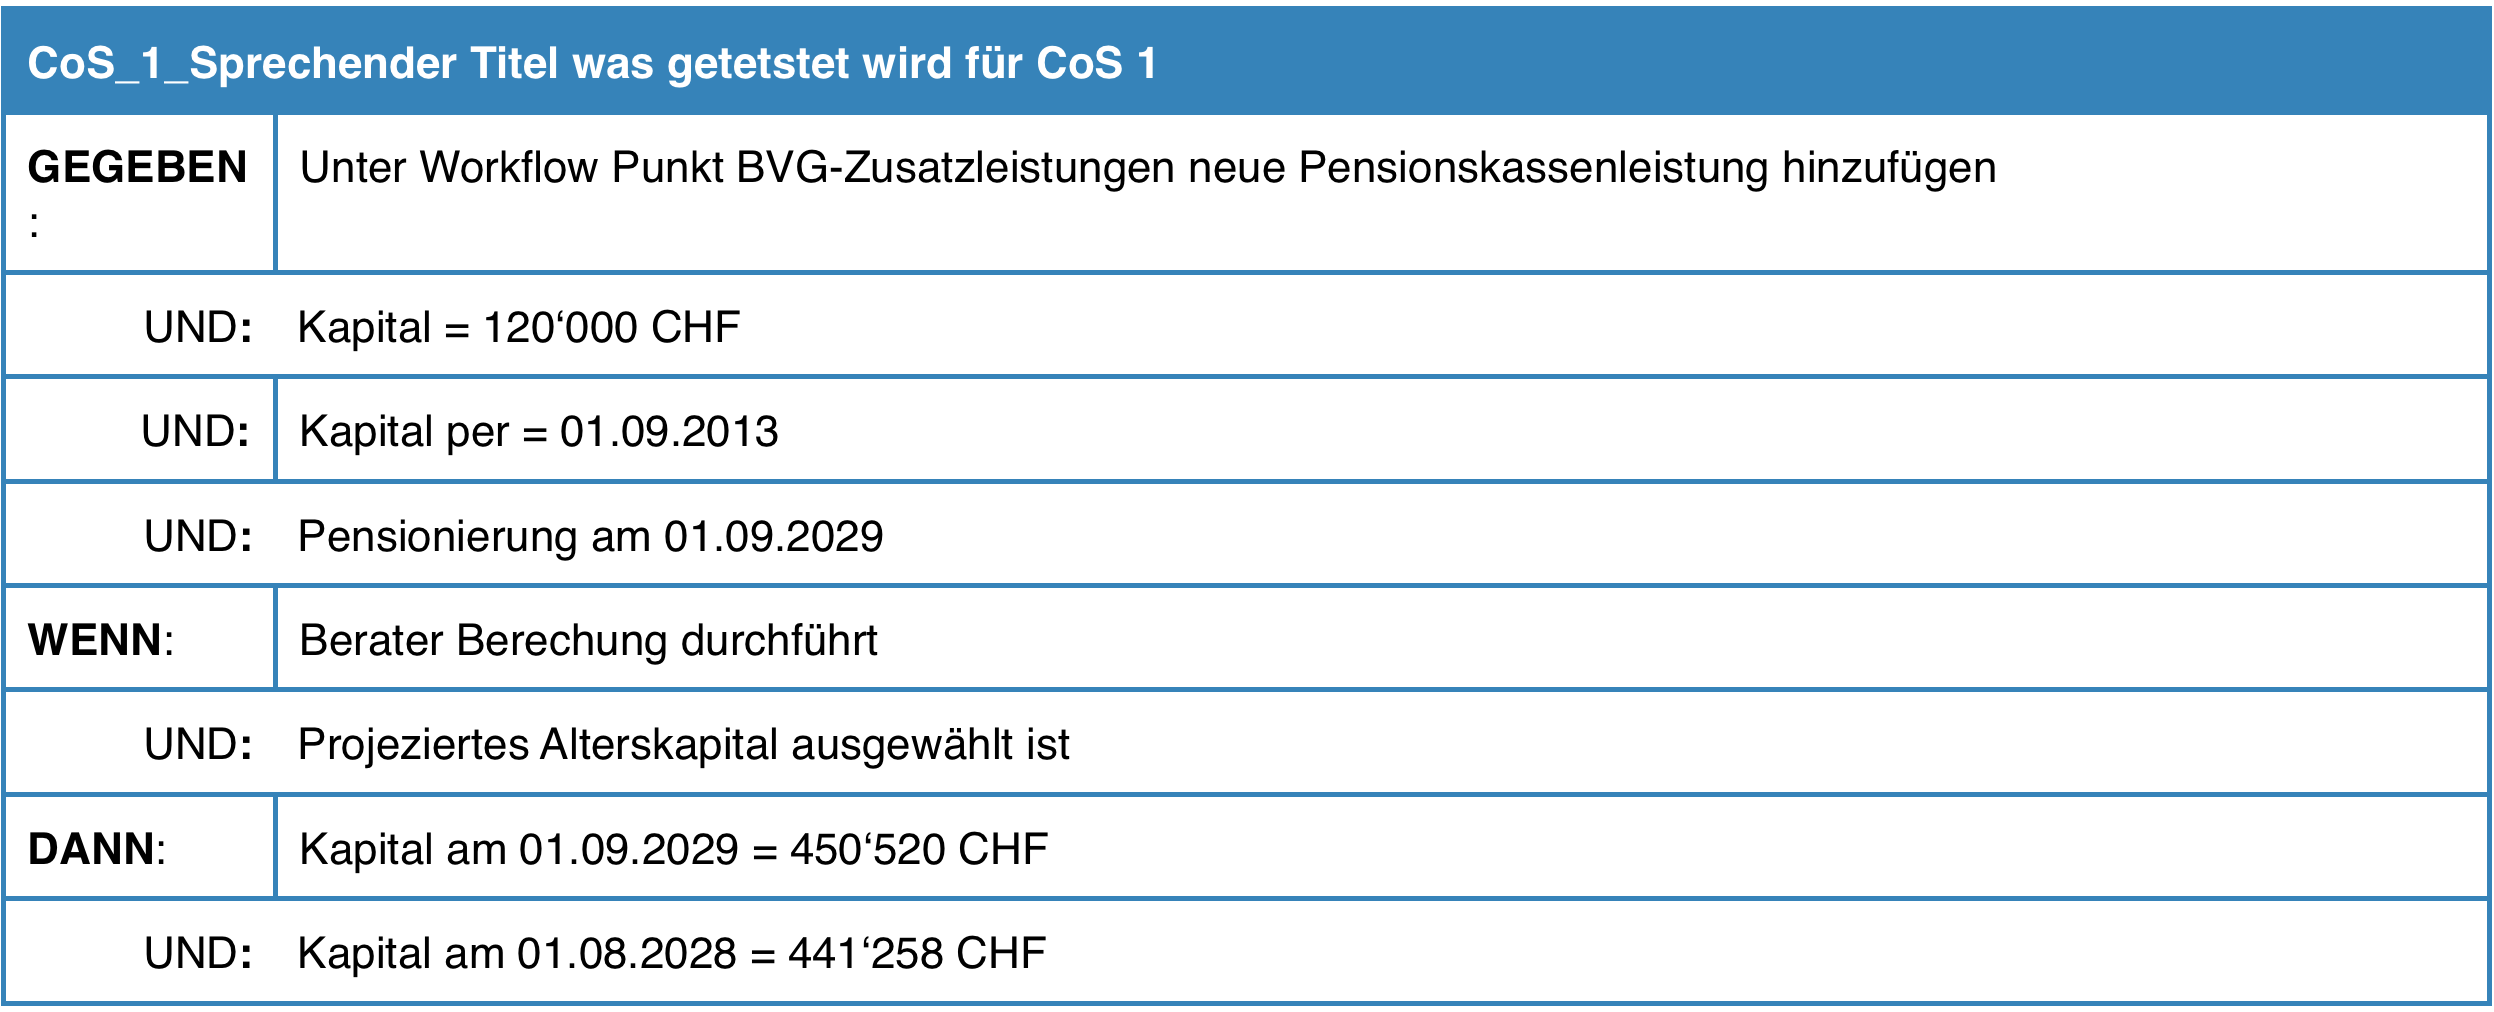
\includegraphics[width=0.9\textwidth]{figures/cos_raiffeisen.png}
  \caption{Muster-COS Tabelle wie sie von den Testfalldesignern verwendet werden.  Angegeben werden Pre- sowie Postconditions und die auszuführenden Aktionen. Der Detailgrad kann erheblich variieren.}
  \label{fig:cos_raiffeisen}
\end{figure}


Auf Seiten der Entwickler, also im Scrum-Team, gibt es keinen dedizierten Tester. Im Entwicklungszyklus fixiert sind nur Unit-Tests. Außerdem werden vom Test-Verantwortlichen auch den Entwicklern manuelle Testfälle zugewiesen die im Rahmen vom Integrationstesting durchgeführt werden.

\subsubsection{Erkannte Schwachstellen in der Qualitätssicherung}
\label{sec:schwachstellen_raiffeisen}
-Viele Beteiligte
-Keine klaren Zuständigkeiten
-Hohe Diversität bei eingesetzten Tools
-Testfalldesign nicht transparent


\subsubsection{Versuch der Qualitätssicherung durch skriptgesteuerte GUI-Tests}

\subsubsection{Aufwendige Wartung von Testdaten}
Tracing von Testdaten und Testfällen (welcher Bereich der Testdaten wird von einem bestimmten Testfall benutzt?). `If data is tightly coupled with behaviour, this can lead to serious maintenance burden' \cite{baker_model-driven_2005} 

%%%%%%%%%%%%%%%%%%%%%%%%%%%%%%%%%%%%%%%%%%%%%%%%%%%%%%%%%%%%%%%%%%%%%%%%

\section{MBT auf Unit-Testebene}
\label{sec:mbt_unit}
\subsection{ModelJUnit}
\label{sec:modeljunit}
ModelJUnit wird von Dr. Mark Utting et al. an der Universität Waikato in Neuseeland entwickelt. Es wird unter der Open Source GNU GPL Lizenz entwickelt und befindet sich zur Zeit in der Version 2.5 \footnote{Homepage des Tools ModelJUnit \url{http://www.cs.waikato.ac.nz/~marku/mbt/modeljunit/}}. Es erlaubt die Modellierung des SUT als endlicher Automat (von hier an FST für \textit{finite state machine}) in Java, Generierung von Testfällen laut spezifiziertem Traversierungsalgorithmus sowie Reporting. Seit Version 2.0 bietet das Tool eine grafische Benutzeroberfläche die die Traversierungskonfiguration ermöglicht und veranschaulicht.\\
\todo{Hier weitermachen aus Utting Buch}
\subsubsection{Traversierung}
\paragraph{Random Walk}
\paragraph{Greedy Walk}
\paragraph{Lookahead Walk}
\paragraph{Quick Walk}


\section{MBT auf Integrationstestebene}
\subsection{Testing von Serviceorientierten Architekturen mittels UML Testing Profile}
\label{sec:utp}
\subsubsection{UML Testing Profile BASICS}

\subsubsection{SOA und Web-Services}
Von Serviceorientierten Architekturen (von hier an \textit{SOA}) verspricht man sich schnelle und einfache Integration innerhalb als auch über Unternehmensgrenzen hinweg. Die Möglichkeit eine Applikation mittels Komposition, maßgeschneidert zu den gegebenen Requirements, zusammenzustellen, ist traditionellen Software-Engineering Methoden oft voraus. Gleichzeitig stellen verschachtelte und unabhängige Strukturen den Tester vor neue Herausforderungen. \\
SOA wird missbräuchlich oft mit Web-Services gleichgestellt. Tatsächlich sind Web-Services nur die häufigste architektonische Grundlage auf der SOA-Applikationen laufen. Die folgende Sektion geht ebenfalls von einer Serviceorientierten Architektur basierend auf Web-Services aus.

\subsubsection{Mapping von Web-Service Elementen auf UML-Diagramme}
Am Beispiel eines Web-Services der per WSDL\footnote{WSDL Web-Service Spezifikationssprache 2.0 \url{http://www.w3.org/TR/wsdl20/}} definiert ist, soll gezeigt werden wie eine Modellierung von Web-Services mittels dem UML-Testing Profile umgesetzt werden kann. \footnote{Sehr ähnlich würde eine Modellierung für RESTful Web-Services basierend auf WADL ausschauen. Hierbei stellt sich aber eine Grundsatzfrage: Eines der Prinzipien von REST ist die Fähigkeit, dass sich ein Web-Service selbst beschreiben kann. Inwiefern trotzdem WADL Dateien gebraucht werden, hängt von der jeweiligen Implementierung ab.} Baker et al. schlagen folgende Vorgehensweise für das Mapping vor\cite{_model-driven_2007}:

\begin{itemize}
\item WSDL Port Types werden zu UML Stereotyp-Klassen gemappt
\item Die Operationen in dieser Klasse stellen die Operationen dar, die der jeweilige Port Type offenbart.
\item Jede Operation hat eine übereinstimmende Request Message. Falls die Operation auch einen Rückgabewert definiert, wird auch dieser abgebildet.
\item Komplexe Typen als auch Enumerationen werden zu stereotypisierten Klassen.
\end{itemize}

\subsubsection{Teststrategie für Web Services}
Im Gegensatz zu herkömmlichen Desktop-Applikationen aus einer Hand, können SOA Web-Services tief verschachtelte Komponenten von verschiedensten Parteien enthalten. Dies erschwert das Testing auf zwei Arten. Erstens können gravierende Qualitätsunterschiede zwischen Web-Services bestehen. Zweitens unterliegen diese benutzten Web-Services eigenen Wartungs- und Änderungsintervallen. Diese Erkenntnisse haben zur Folge, dass an die Teststrategie für Web-Services folgende zusätzliche Anforderungen gestellt werden:

\begin{itemize}
\item Tests müssen schnell und oft durchführbar sein (nämlich dann wenn eine Komponente geändert wird): \textit{On-Demand Testing}.
\item Gleichzeitig müssen die Tests kompakt und schnell wartbar sein (ähnlich Unit-Tests).
\item Web-Services sollen einzeln getestet werden können. Dies ermöglicht nicht nur eine gewisse Modularität, die zu einer hohen Test-Geschwindigkeit beiträgt sondern erleichtert auch die Fehlersuche einem negativen Testdurchlauf.
\end{itemize}

Web-Services müssen \textit{mehrdimensional} getestet werden\cite{_model-driven_2007}. Das bedeutet, ein modellbasierter Testfall soll alle Port Types, die der Service zur Verfügung stellt, kombiniert mit allen Operationen die jeder Port Type anbietet, prüfen. Als Testdaten müssen die Equivalenzklassen aller Datentypen die der Web-Service anbietet identifiziert werden.

\subsubsection{Beispielhafte TestSuite eines SOA Web-Services}
\todo{UML-Diagramme (und evt. WSDL)aus Buch einbinden} In diesem Beispiel wird ein Service einer Bücherei oder einer Buchhandlung herangezogen. Einfachheitshalber bietet dieser Service nur einen Port Type (LibraryService) an. Auf diesem werden drei Operationen angeboten (search, reserve, fetch). Ein Client kann ein Element aus dieser Bücherei also suchen und basierend auf seinem Status-Parameter handeln. Das Element kann sofort verfügbar, später verfügbar und nicht lokal verfügbar sein.\\

Um die angesprochene mehrdimensionale Abdeckung zu gewährleisten bietet das UML Testing Profile das Konzept der Data Pools.\todo{Ref zu Kapitel UTP}. Der DataPool stellt das kartesische Produkt dar, dass aus Operationen und Datenelementen gebildet wird. Nun kann ein Testtreiber auf diesem DataPool operieren und auf Testfalldiagramme (UML-Sequenzdiagramme) referenzieren.\\
Anhand von diesem einfachen Beispiel wird sichtbar, dass das UML Testing Profile sinnvolle Erweiterungen definiert, die die Modellierung von modernen SOA-Applikationen vereinfachen. Data Pools visualisieren die Abdeckung von Äquivalenzklassen und modularisierte Sequenzdiagramme erlauben die Modellierung von umfangreichen Testfällen. 


\subsubsection{Ausfühhrung von UTP Tests mittels JUnit}
Agile Praktiken haben die Wahrnehmung der die Wichtigkeit des Unit-Tests erhöht\cite{_model-driven_2007}. Ansätze wie \textit{Test-First} sind in diesem Umfeld besonders populär und der klassische Unit-Test spielt dabei eine zentrale Rolle. Dieses Kapitel geht davon aus, dass der Leser mit den Grundlagen von JUnit 4\footnote{Webseite des JUnit Projekts \url{http://junit.org/}} vertraut ist.\\

Zum Zeitpunkt dieser Arbeit, gibt es keine Tool mit welchem die automatische Generierung von JUnit-Testfällen aus UTP-Modellen erlaubt. Das bedeutet, um MBT basierend auf UTP-Modellen in einem realen Umfeld zu betreiben, muss das Mapping manuell gemacht werden. Baker et al. schlagen dabei folgende Vorgehensweise vor\cite{_model-driven_2007}:

\begin{table}[h]

\centering
\begin{tabular}
{ | l |p{9cm}|} \hline
\textbf{UTP} & \textbf{JUnit} \\ \hline
SUT                       & Kein direktes Mapping nötig. Jede Klasse im \textit{Classpath} kann angesprochen und getestet werden   \\ \hline
Kontext                   & Kein direktes Mapping. JUnit kann auf den realen Kontext des SUT zugreifen. Aufwände außerhalb der JUnit-Programmierung sind nötig um alternative Konfigurationen zu testen \\ \hline
Ablauf         			  & JUnit bietet die Klasse \textit{org.junit.runner.Runner} um feingradige Einstellungen am Testablauf zu machen. \\ \hline
Sheduler                  & Alle vom Java-Umfeld bereitgestellten Möglichkeiten des Shedulings sind einsetzbar (auch \textit{org.junit.runner.Runner} bietet Sheduling-Optionen) \\ \hline
Test configuration        & Implizit gegeben in JUnit, durch die direkte Einbindung der Klassen die getestet werden. \\ \hline
Test objective            & Dieses Konzept bietet JUnit nicht. Methoden können höchstens mit entsprechenden Kommentaren versehen werden.\\ \hline
Test case                 & Eine Methode die mit der Annotation \textit{@Test} versehen ist. \\ \hline
Test invocation           & Aufrufe der Methoden die mit \textit{@Test} annotiert sind. Üblicherweise durch einen Test-Runner. \\ \hline
Arbiter                   & Die Klassen \textit{org.junit.runner.Runner} und \textit{org.junit.runner.notification.RunListener} entscheiden über die Bewertung des Ausgangs eines Testfalls. Diese Klassen können bei Bedarf auch erweitert werden. \\ \hline
Verdict                   & Vordefinierte Testfallergebnisse sind \textit{pass},\textit{fail} und \textit{error}. Auch diese Klasse kann um mehr Funktionalität erweitert werden. \\ \hline
Defaults                  & JUnit bietet keinen vergleichbaren Mechanismus.  \\ \hline
Validation action         & Validation Actions mappen auf die vielfältigen Methoden der Klasse \textit{org.junit.Assert} \\ \hline
Stimulus and observation  & Keine entsprechende Funktionalität in JUnit. \\ \hline
Logging concepts          & Im Java-Umfeld gibt es verschiedenste Logging-Frameworks die mit JUnit verwendet werden können. \\ \hline
Testdatenmanagement: Data pools & \textbf{Es sind keine entsprechenden Konzepte in JUnit eingebaut.} \\ \hline
Testdatenmanagement: Wildcards  & Es sind keine entsprechenden Konzepte in JUnit eingebaut.\\ \hline
Timer                     & Es sind keine entsprechenden Konzepte in JUnit eingebaut. \\ \hline
Timezone                  & Es sind keine entsprechenden Konzepte in JUnit eingebaut. \\ \hline
Deployment       & JUnit fügt sich im Deployment Prozess sehr gut ein. \\ \hline
\end{tabular}
\caption{Mapping von UTP zu JUnit}
\end{table}

\todo{UTP zu JUnit Code Beispiel einfügen eventuell}
UTP wurde entwickelt um mit JUnit zusammenzuspielen\cite{_model-driven_2007}. Tatsächlich lassen sich viele Konzepte gut von UTP-Modellen nach JUnit übertragen. Gleichzeitig hat die Ausführung von UTP-Testfällen in JUnit gravierende Schwächen.

\paragraph{Manuelles Mapping} Es hat sich in den Jahren, seit das UML Test Profile veröffentlicht wurde, keine Community um die Nutzung und Entwicklung von Tools gebildet. Die Eigenentwicklung eines JUnit-Testfallgenerators kann im Umfeld von großen Softwareprojekten sinnvoll sein. Gleichzeitig bleibt der Aufwand um den sogenannten \textit{glue code} zu schreiben (also die Implementierungsdetails innerhalb der Testmethoden).\\
Jedenfalls können durch einen manuellen Eingriff neue Fehler entstehen. Ein Modell mittels Testfällen umzusetzen ist kein trivialer Vorgang und erfordert genaue Kenntnisse des Frameworks sowie des SUT. Ob sich die Modellierung und die Aufwände für die Umsetzung in JUnit-Testfällen lohnt, lässt sich schwer feststellen. Faktisch bietet die Modellierung als UTP-Diagramm zwar strukturierte Testfälle (verglichen mit der Ad-Hoc Entwicklung von JUnit-Testfällen) aber keine weiteren Qualitätsmetriken. Entwicklungsumgebungen und statische Code-Analyse Tools können die Abdeckung von JUnit-Testfällen eruieren, diese ist in agilen Softwareprojekten aber ohnehin schon sehr hoch. Ein modellbasierter Ansatz kann hier wenig belegbare Qualitätsvorteile schaffen.

\paragraph{Keine Unterstützung der Testdatenmangementkonzepte}
Vor allem das \textit{Data Pool} Konzept von UTP ist eine Notwendigkeit für datenintensive Applikationen. Datengetriebene Testfälle müssen durch ein flexibles und zuverlässiges Konzept gestützt werden. Auch hier müsste eine Eigenentwicklung gemacht werden. Diese ist aber nicht nur aufwendig sondern stellt sich auch die Frage der Zukunftssicherheit. Kann das Modul zum Testdatenmanagement mit anderen Technologien verwendet werden oder ist es zu stark auf UTP zugeschneidert?

\subsection{Schnittstellentests mit Graphwalker}
\label{sec:graphwalker}
Graphwalker\footnote{Graphwalker 3 Website inklusive Dokumentation \url{www.graphwalker.org}} ist ein Open Source MBT-Tool zur Online- und Offline Generierung von Testsequenzen aus Endlichen Automaten (siehe Abschnitt \ref{sec:fsm}) sowie Erweiterten Endlichen Automaten (EFSM).Graphwalker ist in Java und JavaScript implementiert und bietet eine Java-API an. Das Graphwalker-Projekt wurde von zwei Entwicklern der Firma Spotify, Nils Olsson und Kristian Karl, gegründet. Bei Spotify, dem marktführenden Musik-Streaming-Service, ist das Tool auch stark im Einsatz. Graphwalker ist zur Zeit (Frühjahr/Sommer 2015) aktiv unter Entwicklung und liegt bereits in der Version 3.0 vor.\\
Graphwalker weicht ab vom herkömmlichen Testfall-Workflow. Das SUT wird in einem Modell (Graph) modelliert und das Testing (also die Traversierung des Graphs) wird vom gewählten Algorithmus und dessen Konfiguration bestimmt. Daraus resultieren lange, unvorhersehbare Testdurchläufe. Die offizielle Dokumentation beschreibt es so:

\begin{quote}
`We do not want to walk the same path every time we execute a test. We want variation, spiced with randomness. This will create a better `test coverage' of the system under test.'\cite{_graphwalker_2015}
\end{quote}

Beim Einsatz in den agilen Entwicklungsteams von Spotify hat sich gezeigt, dass diese Testdesign-Philosophie sehr gut in die kurzen Entwicklungsiterationen passt. Weiters eignen sich die simplen FSM-Diagramme sehr gut um Feedback von Stakeholdern einzuholen, weil sie auch ohne technischen Hintergrund verständlich sind.

\subsubsection{Modellierungs-Syntax}
Graphwalkers Modellierungssprache basiert nicht auf UML, weil die Autoren glauben, dass Tester vom großen Funktionsumfang von UML nicht brauchen und abgeschreckt werden. Stattdessen setzt Graphwalker auf GraphML\footnote{Website des GraphML Projekts \url{graphml.graphdrawing.org}}. GraphML setzt nicht auf eine proprietäre Syntax sondern basiert auf herkömmlichen XML-Dateien und wird unter der \textit{Creative Commons Attribution 3.0}-Lizenz entwickelt.\\
Zur Erstellung von Modellen in GraphML, mit denen Graphwalker umgehen kann, eignet sich jedes Tool, das GraphML-Dateien exportieren kann. Das von den Entwicklern empfohlene Tool ist \textit{yEd}\footnote{Website der Firma yWorks und des yEd Graph Editors \url{http://www.yworks.com/en/products/yfiles/yed/}}, welches völlig kostenlos verwendet werden kann. yEd bietet eine simple Benutzeroberfläche und für die Erstellung von Modellen für Graphwalker ist nahezu kein Einarbeitungsaufwand vorhanden.\\
Modelle in Graphwalker sind gerichtete Graphen. Knoten repräsentieren einen Zustand in dem sich das SUT befindet. Kanten beschreiben die Aktion die zu einem bestimmten Zustand führen. Graphwalker ignoriert grafische Attribute der Modelle wie Farbe und Liniendicke der Elemente. Üblicherweise finden in den Knoten die Überprüfungen (\textit{Assertions}) und in den Kanten die Befehle (Klicks, Schnittstellenaufrufe...) statt. Kanten müssen in Graphwalker genau eine Richtung haben. Es folgt eine kurze Beschreibung der Möglichkeiten, die die Syntax von Graphwalker bietet um die Traversierung der Graphen, und damit der Testfälle, zu beinflussen.

\paragraph{Start vertex} Wenn ein Startknoten definiert wird, darf es nur genau einen geben. Es ist aber nicht obligatorisch einen Startknoten zu definieren.

\paragraph{Guards} Auf Kanten könnten sogenannte \textit{Guards} definiert werden. Dabei handelt es sich um einen Konditionalmechanismus. Wenn das Konditional zu wahr evaluiert, wird die Kante traversierbar. Ein \textit|{Guard} wird mittels eckigen Klammern beschrieben.
\begin{verbatim}
[loggedIn == true]
\end{verbatim}

\paragraph{Actions} Auch \textit{Actions} sind nur auf Kanten definierbar. Hierbei handelt es sich um Code in JavaScript-Syntax der zur Zeit der Traversierung ausgeführt wird. Die in \textit{Actions} durchgeführten Zuweisungen werden in \textit{Guards} abgefragt.

\paragraph{Keywords} Diese Schlüsselwörter beschreiben keine Eigenschaften des SUT, sondern dienen nur der Usability und Modularität der Modelle.


\begin{itemize}
\item Start: Beschreibt den Startknoten
\item BLOCKED: Dieser Knoten oder diese Kante wird bei der Traversierung aus dem Graphen entfernt.
\item SHARED: Dient zur Modularisierung. Wenn Graphwalker bei der Traversierung auf einen mit SHARED annotierten Knoten trifft, passiert ein Sprung in ein anderes Modell mit dem selben SHARED-Bezeichner.
\item INIT: Dient zur Initialisierung von Datenfeldern die im Modell genutzt werden. Nur Knoten können mit dem INIT-Schlüsselwort versehen werden.
\end{itemize} 

\paragraph{Modularisierung der Modelle}
Das SUT kann in Graphwalker mittels mehreren Modellen abgebildet werden. Dies hat mehrere Vorteile. Einerseits vereinfacht die Modularisierung eines großen Modells die Les- und Wartbarkeit. Andererseits wird dadurch die Wiederverwendbarkeit von Teilen der Funktionalität ermöglicht. Ein klassisches Beispiel ist ein Login-Workflow. Dieser kann oft zu mehreren Zeitpunkten bzw. an mehreren Stellen im SUT erfolgen. Statt das Modell aufzublähen oder mit zahlreichen Beziehungen schlechter lesbar zu machen, kann auf eine andere GraphML-Modelldatei verwiesen werden.\\
Graphwalker ermöglicht dies mit Sprüngen in andere Modelle. Wenn es bei der Traversierung auf einen Knoten mit dem Schlüsselwort \textit{SHARED} und einem Bezeichner stößt, kann ein Sprung in ein anderes Modell erfolgen, das einen Knoten mit dem selben Bezeichner hat (siehe Abbildung \ref{fig:gw_multiple_models}). Wenn nun mehrere Kanten zur weiteren Traversierung in Fragen kommen, entscheidet der Zufall ob in das andere Modell gesprungen wird.\\
Weiters ist zu erwähnen, dass die Modelle nicht einfach nur verflacht (\textit{flattening}) werden. Das bedeutet, dass die Modelle unabhängige Gültigkeitsbereiche haben. Die Traversierung erfolgt also in einem eigenen Kontext.

\begin{figure}[h] 
  \centering
     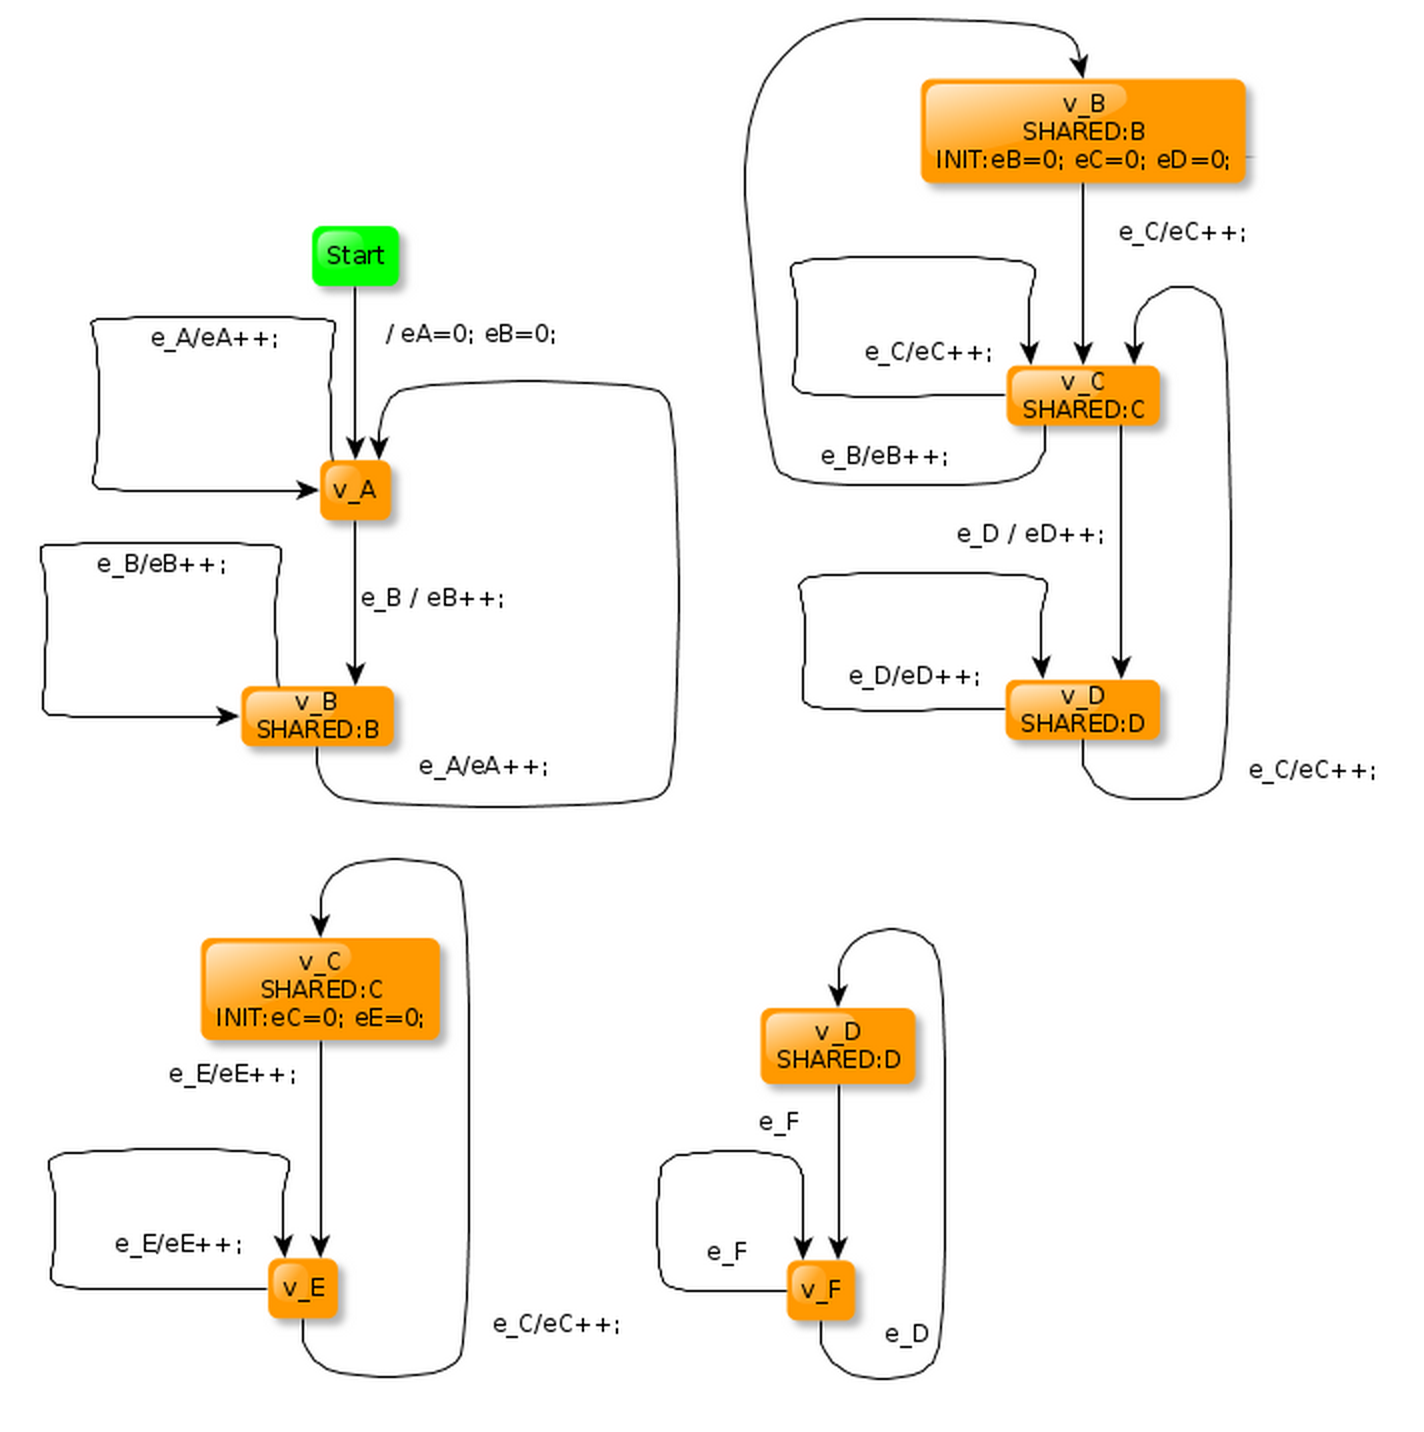
\includegraphics[width=0.9\textwidth]{figures/gw_multiple_models.png}
  \caption{Vier einzelne Modelle die bei einer Traversierung (ausgehend vom Startknoten in Grün) erreicht werden können. Bei den Knoten die mit \textit{SHARED} gekennzeichnet sind kann ein Sprung (und auch ein Sprung zurück) erfolgen. Die Variablen mit den selben Bezeichnern in den Modellen B und C befinden sich in unabhängigen Gültigkeitsbereichen.\cite{_graphwalker_2015}}
  \label{fig:gw_multiple_models}
\end{figure}

\paragraph{Traversierung der Modelle}  
Wie im ursprünglichsten Sinn des modellbasierten Tests, kennt Graphwalker das Konzept der Testfälle nicht. Das SUT wird als gesamtes oder nur zu Teilen modelliert und das Testing wird durch die Auswahl eines Traversierungsalgorithmus angestoßen. Da die meisten Traversierungsalgorithmen von einer randomisierten Variante abhängen, wird das SUT bei jedem Testdurchlauf leicht unterschiedlich traversiert und damit getestet.\\
Durch die Modellierung des Modells und der Auswahl sowie Einstellung eines Traversierungsalgorithmus kann also bestimmt werden wie das SUT getestet werden soll. Dabei bietet Graphwalker bereits verschiedenste Algorithmen an, die sich für unterschiedliche Testzwecke eignen. Die meisten dieser Algorithmen basieren auf bekannten Graph-Algorithmen und bieten, durch die quelloffene Entwicklung, volle Transparenz gegenüber dem Tester.

\subparagraph{Schnelle Traversierung - Smoke Tests}
Vor allem während der Testfallentwicklung und um sogenannte \textit{Smoke Tests} zu machen eignet sich der A*-Algorithmus von Graphwalker. Er basiert auf dem bekannten A*-Suchalgorithmus von Hart et al. \cite{hart_formal_1968}. Dabei wird also ein zu findender Knoten angegeben, meist ein Knoten der das Ende eines Workflows darstellt. Graphwalker durchschreitet das Testsystem dann in einem möglichst kurzen Pfad, wobei die zugrundeliegende Suchheuristik bei jedem Schritt angepasst wird.

\begin{verbatim}
@Test
public void runSmokeTest() {
  new TestBuilder()
    .setPathGenerator(new AStarPath(new ReachedVertex("v_Browse")))
    .execute();
    
}
\end{verbatim}


\subparagraph{Traversierung basierend auf Pfadabdeckung - Funktionaler Test}
Umfangreiche funktionale Tests einer komplexen Applikation, wie sie beispielsweise über Nacht gemacht werden, können mit Graphwalker unter anderem durch eine Zufallstraversierung mittels Angabe der gewünschten Pfadabdeckung realisiert werden. Falls eine einhundertprozentige Abdeckung eingestellt wird (wie im folgenden Beispiel), wird das Modell vom Startknoten (falls angegeben) aus traversiert bis jede begehbare Kante traversiert wurde. Gegegebenenfalls werden weitere Durchläufe gestartet, falls es Teilgraphen gibt die vom designierten Startknoten nicht erreichbar sind. 

\begin{verbatim}
@Test
public void runFunctionalTest() {
  new TestBuilder()
    .setPathGenerator(new RandomPath(new EdgeCoverage(100)))
    .execute();
    
}
\end{verbatim}

\subparagraph{Traversierung mit Zeitangabe - Last- und Performance Test}
Mit einer Traversierung der Modelle mit Zeitangabe kann Graphwalker für Last- und Performance-Tests benutzt werden. Durch die Leichtgewichtigkeit von Graphwalker können Traversierungen auch parallel gestartet werden um damit nicht unerhebliche Last auf ein Software-System zu bringen. Um eine Traversierung mit Zeitangabe gestartet wird ein Traversierungsalgorithmus (zum Beispiel die Klasse RandomPath) und ein Zeitlimit angegeben.\\
Graphwalker bietet aber keine Möglichkeit Metriken während des Durchlaufs zu erfassen. Diese Funktionalität muss durch andere Bibliotheken realisiert werden, was aber sehr einfach möglich ist.
\begin{verbatim}
@Test
public void runFunctionalTest() {  
  new TestBuilder()
    .setPathGenerator(new RandomPath(new TimeDuration(30, TimeUnit.SECONDS)))
    .execute();
}
\end{verbatim}


\subsection{Einbindung SoapUI/HP UFT}


\section{MBT auf Systemtestebene und Test non-stop}
\subsection{Manuelle Systemtests anhand von Modellen}
\subsection{Automatisierte MBT GUI-Tests (GUITAR)}
\subsection{Automatische Modellgenerierung auf Produktionsebene (LearnLib)}
%%%%%%%%%%%%%%%%%%%%%%%%%%%%%%%%%%%%%%%%%%%%%%%%%%%%%%%%%%%%%%%%%%%%%%%%
\chapter{Neuartige modellbasierte Teststrategie für große agile Projekte}
\label{sec:results}
%%%%%%%%%%%%%%%%%%%%%%%%%%%%%%%%%%%%%%%%%%%%%%%%%%%%%%%%%%%%%%%%%%%%%%%%

Aufbauend auf den Erkenntnissen der Fallstudie (siehe Abschnitt \ref{sec:fallstudie}) wurde eine neuartige modellbasierte Teststrategie entwickelt um komplexe Softwaresysteme in agilen Projekten zu testen. Diese Strategie hat unter anderem folgende Eigenschaften und zielt auf die, in Abschnitt \ref{sec:schwachstellen_raiffeisen}, beschriebenen Schwachstellen ab:

\begin{enumerate}
\item Einfachere Einbindung der Fachbereiche und Minimierung der Spezifikations-/Implementationslücke.
\item Minderung des Wartungsaufwandes für die Testlogik
\item Eliminierung der Notwendigkeit eine hohe Anzahl von einzelnen Teställen zu definieren
\item Visualisierung der Spezifikation und Bewusstmachung des potenziellen Testaufwandes
\item Minimierung der Abhängigkeit zu einem Werkzeug durch Wahl eines quelloffenen Tools
\item Möglichkeit des punktuellen Einsatzes bzw. der inkrementellen Einführung
\item Erhöhung der Testabdeckung und damit Erhöhung der Qualität des Softwaresystems
\end{enumerate}

Im folgenden wird die genannte Teststrategie näher beschrieben. Abbildung \ref{fig:testarchitektur} stellt die Testarchitektur konzeptuell dar.

\begin{figure}[h] 
  \centering
     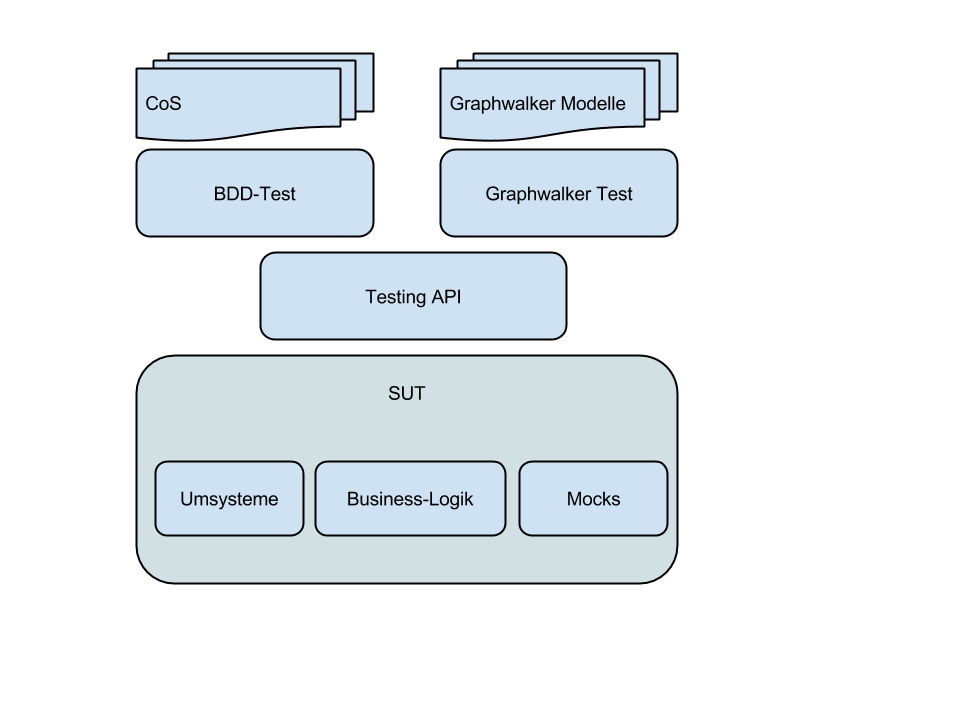
\includegraphics[width=1.0\textwidth]{figures/Testarchitektur-MBT-BDD-COS.png}
  \caption{Am oberen Ende der Testarchitektur liegen die \textit{Conditions of Satisfiction}, die vom Kunden oder Fachbereich definiert werden. Sie dienen als Basis für die BDD-Tests. Graphwalker operiert auf Modellen im graphml-Format. Dabei können beide Frameworks entweder auf die Testing API zugreifen oder direkt auf das SUT.}
  \label{fig:testarchitektur}
\end{figure}

\section{Aufbau der Teststufen}
Im Sinne von Test-First und einer hohen Priorisierung von Unit-Tests soll der Fokus des Testings auf drei Arten von Tests liegen:

\begin{itemize}
\item Eine breite Basis von Unit-Tests mit hoher Abdeckung
\item Modellbasierte Systemtests auf mehreren Ebenen mit direkter Verbindung zu Anforderungen/Changes
\item Manuelle System- und Abnahmetests
\end{itemize}

In Anlehung an Linz\cite{linz_testing_2014} (und mit dem Verweis auf die Diskussion in Abschnitt\ref{sec:discussion_unit}) soll die Unit-Test Ebene in Scrum-Projekten am breitesten sein\todo{Test PYRAMIDE einfügen}. Dies erscheint mit Hinblick auf die vielen kurzen Iterationen, die das Softwaresystem stark verändern, auch logisch. Unit-Tests lassen sich, weil sie am entwicklungsnächsten sind, auch am schnellsten modifizieren. Obwohl Unit-Tests einzelne Komponenten in Isolation testen, müssen sie zumindest eine verlässliche Aussagen treffen können, dass ebenjene Komponente ordnungsgemäß operiert. Diese Aussage wird möglich durch eine hohe Codeüberdeckung in Verbindung mit sorgfältig designten Testfällen. Auch auf Unit-Testebene gelten Best-Practices und Methodiken für hochqualitative Testfälle, wie sie Spillner und Linz beschreiben\cite{spillner_software_2014}. Die Besonderheit im Unit-Testing dieser Teststrategie liegt im Einsatz eines Behaviour-Driven-Testing\cite{chelimsky_rspec_2010} Frameworks und einer Testing-API. Für erstere Komponente existieren einige frei erhältliche Vertreter\footnote{Im Java-Umfeld bekannt sind die Frameworks \textit{jBehave} \url{http://jbehave.org/} und \textit{cucumber} \url{https://cucumber.io/}}. In der Raiffeisen-Fallstudie wurde aber eine Eigenentwicklung als \textit{Proof of Concept} gemacht (siehe Abschnitt \ref{sec:bdd} für eine kurze Erläuterung). Die erwähnte Testing-API (siehe Abschnitt \ref{sec:testing_api}) bietet Schnittstellen zu Programmlogik und Umsystemen.\\
Im Sinne dieser Arbeit steht der modellbasierte Anteil der Teststrategie im Mittelpunkt. Es soll aber erwähnt sein, dass keine zwei Softwareprojekte gleich sind und sich die Gewichtungen der Testmethodiken im Detail unterscheiden \textit{sollten}! Der modellbasierte Anteil basiert technisch ausschließlich auf quelloffenen Werkzeugen. Graphwalker (die Funktionsweise des Graphwalker-Frameworks wird in Abschnitt \ref{sec:graphwalker} erklärt) funktioniert als Testtreiber der das SUT systmatisch durchläuft. Welche bzw. welche Art von Schnittstellen in das SUT greifen und es bedienen bleibt völlig offen und muss an die eigenen Bedürfnisse angepasst werden. Bei Applikationen mit GUI (oder wenn über die GUI \textit{End-to-End} Tests gemacht werden sollen) dann könnte zum Beispiel Selenium\footnote{Webseite des Selenium-Projekts \url{http://www.seleniumhq.org/}} eingesetzt werden. Tests auf Schnittstellenebene könnten durch SoapUI\footnote{ Offizielle Webseite von SoapUI \url{http://www.soapui.org/}} oder REST-assured\footnote{Code-Repository von REST-assured \url{https://code.google.com/p/rest-assured/}} angetrieben werden. Auch mächtigere proprietäre Werkzeuge können als Teil dieser Graphwalker-Teststrategie verwendet werden, sofern sie eine Schnittstelle zum Aufruf aus Java-Code besitzen und die Ergebnisse in irgendeiner Art und Weise (bevorzugt als JUnit-Report) zurückliefern können (dieser Ansatz wurde in der Fallstudie nicht erprobt und wird deshalb nicht näher erläutert). Außerdem können Graphwalker-Modelle nicht nur Workflows darstellen die auf GUI-Ebene ablaufen. Genauso vorstellbar sind Operationen die auf Schnittstellenebenen passieren (z.B. Operationen auf Datenbanken oder Web-Services). Bei solchen Tests macht es Sinn eine stabile Zwischenschicht, die Testing-API, einzubauen die wiederrum auf die darunterliegenden Systeme zugreift. Der Aufwand zur Erstellung der API rechtfertigt sich weil auch BDD-Unit-Tests darüber in das SUT greifen.\\
Zuletzt bleiben aber auch manuelle Tests ein wichtiger Bestandteil der Teststrategie. Einerseits sind das Abnahmetests bei Neuentwicklungen beziehungsweise bei modifizierten Teilen des Systems und andererseits auch Regressionstests die geschäftskritische Teile des Systems überwachen.

\section{Details der Teststrategie und Architektur}

\subsection{Behavior Driven Testing Framework}
\label{sec:bdd}
Der Fokus dieser Arbeit liegt auf dem modellbasierten Teil der Teststrategie, trotzdem soll erläutert werden welche Rolle \textit{Behavior Driven Testing} im Gesamtbild spielt. In der Softwareentwicklung, und vor allem in großen Projekten, wird viel Aufwand betrieben um Anforderungen von Domänenexperten möglichst nahtlos in die Implementation einfließen zu lassen. Abhängig vom Projekt liegen zwischen diesen Anforderungen und der endgültigen Realisierung mehrere Stufen und Parteien. Die Einführung von BDT zielt also vor allem auf die bereits erwähnte Minimierung der Spezifikations-/Implementationslücke. Auch MBT optimiert diesen Umstand (wie in Abschnitt \ref{sec:mbt_vorteile} beschrieben), aber es hat sich herausgestellt, dass es nicht zielführend ist für jede Anforderung den modellbasierten Ansatz anzuwenden.\\
Behavior Driven Testing, im weiteren Sinne bekannt als Behavior Driven Development, wurde ursprünglich von Dan North beschrieben. Er publiziert und diskutiert über BDD auf einer von ihm verwalteten Webseite\cite{north_official_2015}. BDD basiert auf drei Grundprinzipien:

\begin{itemize}
\item Domänenexperten und Techniker sollen auf einer Ebene kommunizieren und über das System mit einem gemeinsamen Vokabular referenzieren.
\item Jedes System muss einen, für alle Parteien, klar erkennbaren unternehmerischen Wert haben. Außerdem muss bewusst werden wie dieser Wert generiert wird.
\item Allen Parteien ist bewusst, dass Analyse, Design und Spezifikation dem Ertragsgesetz unterliegen. Das heißt ab einem gewissen Punkt macht es keinen Sinn mehr Ressourcen zu investieren weil die Wertschöpfung abfällt.
\end{itemize}

Aus Sicht des Domänenexperten (im Fallbeispiel ein Bankberater und in Vertretung dessen der Fachbereich) wird eine Anforderung folgendermaßen spezifiziert: 

\begin{quote} Als \textbf{ROLLE} fordere ich \textbf{ETWAS} und gewinne dadurch \textbf{NUTZEN} \end{quote}

Diese Nähe zur fachlichen Formulierung (im gleichen Vokabular) will man in der Entwicklung nutzen um der Spezifikation so nah wie möglich zu kommen. In der Fallstudie hat sich herausgestellt, dass die erwähnten CoS-Tabellen (siehe Abschnitt \ref{sec:fallstudie}) schon recht genau solchen BDD-Anforderungen entsprechen. Auch sie beschreiben, ausgehend von einem Ausgangszustand welche Paramater zu einem bestimmten Endzustand führen sollen. Eingangs erwähnte BDD-Frameworks benutzen die selbe Struktur um Tests zu definieren. Es lag also nahe diesen Ansatz zu verfolgen, bestehende Vorgehensweisen nicht grundlegend zu verändern und gleichzeitig bessere Spezifikationen zu schaffen. Gleichzeitig bestand in der Fallstudie der Wunsch nach mehr automatischen Regressionstests die genau jene CoS prüfen. Mehrere Problemfelder wurden identifiziert die mit dem Einsatz von Behavior Driven Testing adressiert werden sollten:


\begin{itemize}
\item \textbf{Präzisierung der Spezifikation.} Spezifikationen in Prosatext und Fachjargon bieten ein hohes Potenzial für Missverständnisse und Ungenauigkeiten. Ein gemeinsames Vokabular und eine universell verständliche Syntax um diese Spezifikationen festzuhalten ist nötig.
\item \textbf{Spezifikationen müssen über lange Zeit überschaubar und prüfbar bleiben.} CoS bleiben über viele Iterationen hinweg gültig. Es kommt aber immer wieder vor, dass sie direkt angepasst werden oder von anderen Weiterentwicklungen betroffen sind und geändert werden müssen. Die von den Fachbereichen verwendeten Storybooks lassen sich zwar versionieren (mittels bekannter Dokumenten-/Codeversionierungs-Tools) aber durch die schiere Größe dieser Dokumente ist es unmöglich festzustellen welche CoS noch befriedigt sind und welche verletzt wurden. Es muss eine Form gefunden werden um CoS kompakt und versionierbar, und für alle an der Entwicklung Beteiligten verständlich, darstellen zu können.
\item \textbf{Einfache und nachhaltige Automatisierbarkeit der Regressionstests.} Aus den verfassten CoS sollen, mit wenig Aufwand, automatisierte Regressionstests entstehen. Neben der einfachen Generierung dieser automatisierten Tests sollen vor allem die Aufwände für Wartung niedrig gehalten werden.
\end{itemize}


Als Proof of Concept wurde ein Behavior Driven Testing Framework namens \textit{FluentCoS} entwickelt, das diese Anforderungen erfüllt und gleichzeitig die oben erwähnten Prinzipien von BDD nicht verletzt. Dabei werden Tests in Java-Code verfasst der sich bewusst sehr verständlich liest. Technisch werden Annotationen verwendet und das Framework stößt JUnit-Tests an. Eine Test-Methode kann folgendermaßen ausschauen:

\begin{lstlisting}[caption={In den Kommentaren kann die CoS als Prosa-Text erklärt werden. Der Methodenname entspricht einer eindeutigen Identifizierung für die CoS. Zentral sind die klar verständlichen Aufrufe an \textit{given}, \textit{when} und \textit{then}. Jeweils das zweite Argument innerhalb dieser Aufrufe entspricht einer Methode der Testing API (siehe Abschnitt \ref{sec:testing_api})},label=lst:shortcode]

/**
 * Es muss fachlich sichergestellt sein, dass ...
 * Lorem Ipsum
 */
@Test
public final void cos_1_Hierarchische_Auflistung_und_Bezeichnung_des_Default_Teilvermoegens_Kontovermoegen() {
		given("Kunde XY fuer Beratung ausgewaehlt", selectCustomer("Peter Mueller"))
			.and("Kunde XY besitzt Produkte des TV's 'Kontovermoegen'", initCustomerAssets())
		.when("Berater fuer Kunde XY den Menuepunkt 'Anlegen Finfox' anklickt", clickMenu())
		.then("Wird das TV 'Kontovermoegen' an erster Stelle gezeigt", assertAccountFirst())
			.and("Der Titel des TV beinhaltet eine eindeutige Nummer", assertUniquePortfolioId())
			.and("Den TV-Typ 'Kontovermoegen'", nop());
}
\end{lstlisting}

Die eindeutige Identifikation als Methodennamen stellt sicher, dass eine unverwechselbare Parallele zwischen schriftlich festgehaltenen CoS und automatisiertem Test hergestellt werden kann. Die Kommentarsektion kann zusätzlich verwendet werden um auf Eigenheiten dieser CoS einzugehen. Im inneren der Methode werden dann Aufrufe mit der Struktur \textit{given} \textit{when} \textit{then} gemacht. Damit entsprechen diese Testfälle dem selben Muster, das Dan North als optimale Anforderungsbeschreibung beschrieben hat (Als \textbf{ROLLE} fordere ich \textbf{ETWAS} und gewinne dadurch \textbf{NUTZEN}). Diese BDD-Testfälle haben die Eigenschaft gut lesbar zu sein und ohne weiteres parsen und transformieren automatisch ausführbar zu sein.\\
Bestehende Frameworks nutzen teilweise eine sogenannte \textit{Cleartext}-Syntax um den Testfall zu definieren. Klarerweise handelt es sich aber nicht um natürlichsprachliches Englisch. Auch diese Syntax muss erlernt werden und wird in einem weiteren Schritt in JUnit-Code übersetzt. Wenn nun nicht-technische Domänenexperten in das Schreiben dieser BDD-Testfälle eingebunden werden sollen, müssen sie sich jedenfalls eine neue Syntax aneignen. Bei der Cleartext-Variante wird aber ein weiterer, potenziell fehleranfälliger, Schritt nötig. Deshalb verzichtet FluentCoS auf diesen Zwischenschritt und arbeitet von Anfang an mit einer code-ähnlicheren Syntax.\\
Wenn nicht-technisches Personal weiterhin nicht eingebunden werden soll, und daher die CoS in Prosatext vorliegen, bevorzugen Entwickler mit Sicherheit eine Syntax die Bekanntem entspricht. Java-Entwickler sind allenfalls mit JUnit vertraut. Dies macht eine Cleartext-Syntax ebenfalls unnötig und spricht für die direkte Verfassung der BDD-Testfälle in Java-Code.\\
Denkbar wäre auch eine Teilung der Verfassung dieser CoS. Da Fachbereiche und Entwickler gleichermaßen Zugriff auf die Versionsverwaltung haben, könnten die Fachbereiche die Klassen und Methoden anlegen. Die von ihnen identifizierten CoS tragen sie ein, heißt sie erstellen eine Methode für jede CoS. Jeweils das erste Argument der \textit{given} \textit{when} \textit{then} Aufrufe verfassen sie (dabei handelt es sich tatsächlich um natürlichsprachliches Deutsch oder Englisch). Diese Dateien werden nun versioniert und den Entwicklern zugänglich. Die Entwickler, welche genaue Kenntnisse über die Testing API bzw. das SUT haben, tragen das zweite Argument ein. Meist ein Aufruf an die Testing API. Im weniger einfachen Fall muss ein CoS umstrukturiert werden bzw. muss die Testing API erweitert werden.\\
Bei der Einführung dieser Methode sollte in kurzer Zeit eine komplette Umstellung auf als BDD-Testfall definierte CoS erfolgen. Wenn Anforderungen in mehreren Formaten und an verschiedenen Stellen liegen führt dies zu Unklarheiten, Frustration (durch erhöhte Suchaufwände) und in weiterer Folge zu einem Abfall der Qualität. Durch die starke Koppelung mit automatisierten Tests werden Anforderungen zwingendermaßen präziser. Damit wird auch Anforderung 1 (siehe oben) erfüllt. Außerdem sind CoS in Code-Form von Natur aus sehr kompakt. Für alle Beteiligten ist schneller greifbar welche CoS bestehen.\\
Gleichzeitig bleiben gewisse Probleme bestehen: Obwohl CoS nun direkt an automatisierte Regressionstest gekoppelt sind, ist nicht garantiert, dass bei Neueinführung eines Features, welches eine CoS betrifft, sofort Alarm geschlagen wird. Wünschenswerterweise schlägt der dazugehörige Testfall zwar fehl aber trotz aller Genauigkeit prüfen CoS nur sehr punktuell und wenige Konstellationen. Unter anderem dieses Problem adressiert die komibinierte Nutzung von Behavior Driven Testing und Model Based Testing (siehe Abschnitt \ref{sec:mbt_results}).

\subsection{Testing API}
\label{sec:testing_api}

\subsection{Modellbasierte Tests mit Graphwalker}
\label{sec:mbt_results}
Die Fallstudie hat gezeigt, dass die Diversität der zu testenden Gesichtspunkte des SUT zu hoch ist um einen allumfassenden Ansatz einzusetzen. Dieser Schluss lässt sich mit Sicherheit auf eine große Anzahl von Softwareprojekten übertragen. Selten lassen sich alle wertgenerierenden Aspekte mit einer Art von Tests prüfen. Auch die hohe Anzahl von beteiligten Personen, ob technisch oder fachlich, suggeriert, dass nicht alle die selben Fähigkeiten und Vorlieben für eine Testmethode an den Tag legen.\\
Diese Beobachtungen legen nahe, ein schlankes und flexibles Werkzeug für den modellbasierten Teil der Teststrategie einzusetzen. Repräsentativ für große agile Softwareprojekte ergaben sich weitere Anforderungen an Werkzeug und Umgebung der modellbasierten Tests:

\begin{itemize} 
\item\textbf{Eignung der Feststellung.} Es sollte mit wenig Aufwänden möglichen sein, die Eignung des Werkzeugs für das Testing des SUT festzustellen. Dies setzt erstens voraus, dass vollwertige Testversionen zur Verfügung gestellt werden. Außerdem muss die Funktionsweise, wie das Werkzeug im Hintergrund agiert, dokumentiert und einsehbar sein. Dies ist bei den wenigsten Werkzeugen der fall. Graphwalker, in gewisser Weise implizit durch seine Quelloffenheit gegeben, ist eine erfreuliche Ausnahme.
\item \textbf{Flexibilität des Modellformats.} Vergleichbar mit der Sprache in der die Skripts eines skriptbasierten Tools vorliegen müssen, sind Modellformate für MBT-Tools strikt vorgegeben. Wie effektiv ein SUT getestet werden kann, hängt massiv von der Mächtigkeit des Modellformats ab.
\item \textbf{Verständlichkeit des Modellformats} Das Modellformat an sich aber auch die Präsentation dessen muss verständlich sein.
\end{itemize}


Modellbasiertes Testen kann immer noch als Randerscheinung im Software-Testing angesehen werden. Die Auswahl an Werkzeugen ist deshalb überschaubar. Gerade deswegen ist es aber schwer diese Werkzeuge miteinander zu vergleichen. Sie unterscheiden sich in ihrer Art erheblich. Manche Hersteller designen ihre Tools als Komplettlösung für das Testing auf mehreren Teststufen. Dieser Komplettlösungsansatz erschwert eine Einführung in ein bestehendes Softwareprojekt. Eine Prüfung auf Eignung muss umso umfangreicher erfolgen. Nach einer Einführung kann schwerer auf eine andere Teststrategie umgeschwenkt werden.\\
Aus entwicklerischer Sicht, ist es wünschenswert die interne Vorgehensweise dieser Werkzeuge zu kennen. Dazu zählen die Möglichkeiten wie das SUT modelliert werden kann aber auch entscheidende Details wie das Testdatenmanagement und die Integrationsfähigkeit in die bestehende Umgebung, da meist auf existierende Infrastrukturen Rücksicht genommen werden muss. Dementsprechend sollte nur mit Zugriff auf Dokumentationen bzw. Testversionen herausgefunden werden können welche Fähigkeiten die Werkzeuge bieten und ob sie sich grundsätzlich in das Projekt integrieren lassen.\\
Wie auch im Abschnitt \ref{sec:notations} theoretisch beschrieben und im Diskussionsabschnitt \ref{sec:discussion_unit} angesprochen, bestehen massive Unterschiede bei Tools und deren Modellformaten. Einen weitverbreiteten Standard gibt es nicht und deshalb stellt sich die Frage des Modellformats bei jeder Einführung von MBT in einem Projekt, natürlich auch in der Fallstudie. Eine Eigenentwicklung ist aus mehreren Gründen nicht ratsam. Erstens ist der Entwicklungsaufwand sehr hoch, da keines der evaluierten Tools die Möglichkeit bietet nur das Format bzw. die Sprache selbst zu definieren. Neben formaler Definition der Sprache und Entwicklung eines Lexers und Parsers müsste also die gesamte restliche Infrastruktur entwickelt werden. Dazu zählt die Traversierungslogik, das Reporting und weitere Komponenten. Zweitens würden auch Eigenentwicklungen auf bekannte Modellierungssprachen setzen und könnten das Rad sozusagen nicht neu erfinden. Der Zugewinn an Funktionalität, den Entwicklungsaufwänden gegenübergestellt, wäre sehr klein.\\

\subsubsection{Entscheidende Eigenschaften von Graphwalker}
Graphwalker funktioniert sehr gut als flexibles Grundgerüst für das modellbasierte Testing und kam in der Fallstudie aufgrund der folgenden Eigenschaften zum Einsatz:

\paragraph{Simples aber mächtiges Modellformat} Wie der Name schon sagt, basiert das Modellformat von Graphwalker auf Graphen (siehe Abschnitt \ref{sec:graphwalker} zu Graphwalker). Es hat sich gezeigt, dass diese Graphen als Modellierungssprache ausreichend ausdrucksstark ist um auch komplexe Systeme zu modellieren. Notationen wie das UML Testing Profile (siehe Abschnitt \ref{sec:utp}) bieten eine Vielzahl von verschiedenen Elementen welche die Modelle mächtiger aber gleichzeitig überladen wirken lassen. Die Semantik der Modelle ist ohne Einschulung kaum greifbar.\\
Graphwalker bietet aber trotzdem genug Funktionalität um die Modelle handhabbar zu machen. Einerseits geht es um die Modularisierung des SUT. Bestimmte Funktionalitäten sind an verschiedenen Stellen im System immer wieder gefordert. Genau wie der zugrundeliegende Quellcode für diese Zwecke modularisiert worden ist, so sollen auch das Modell des SUT modularisierbar sein. Graphwalker erlaubt daher die Aufteilung des Modells in mehrere Teile und die Markierung eines Knoten als \textit{Sprungknoten}. Von diesen Knoten aus kann bei der Traversierung in eine andere Modell-File gesprungen werden. Dort wird die Traversierung fortgesetzt und, falls vorhanden, über einen weiteren \textit{Sprungknoten} zurückgekehrt.

\paragraph{Transparente Vorgehensweise} Code-Generierung, Traversierung

%%%%%%%%%%%%%%%%%%%%%%%%%%%%%%%%%%%%%
\subsubsection{Möglichkeiten zur Modellierung - Arten von fachlichen Modellen}
%%%%%%%%%%%%%%%%%%%%%%%%%%%%%%%%%%%%
\paragraph{Workflow-Modellierung}

\begin{figure}[h] 
  \centering
     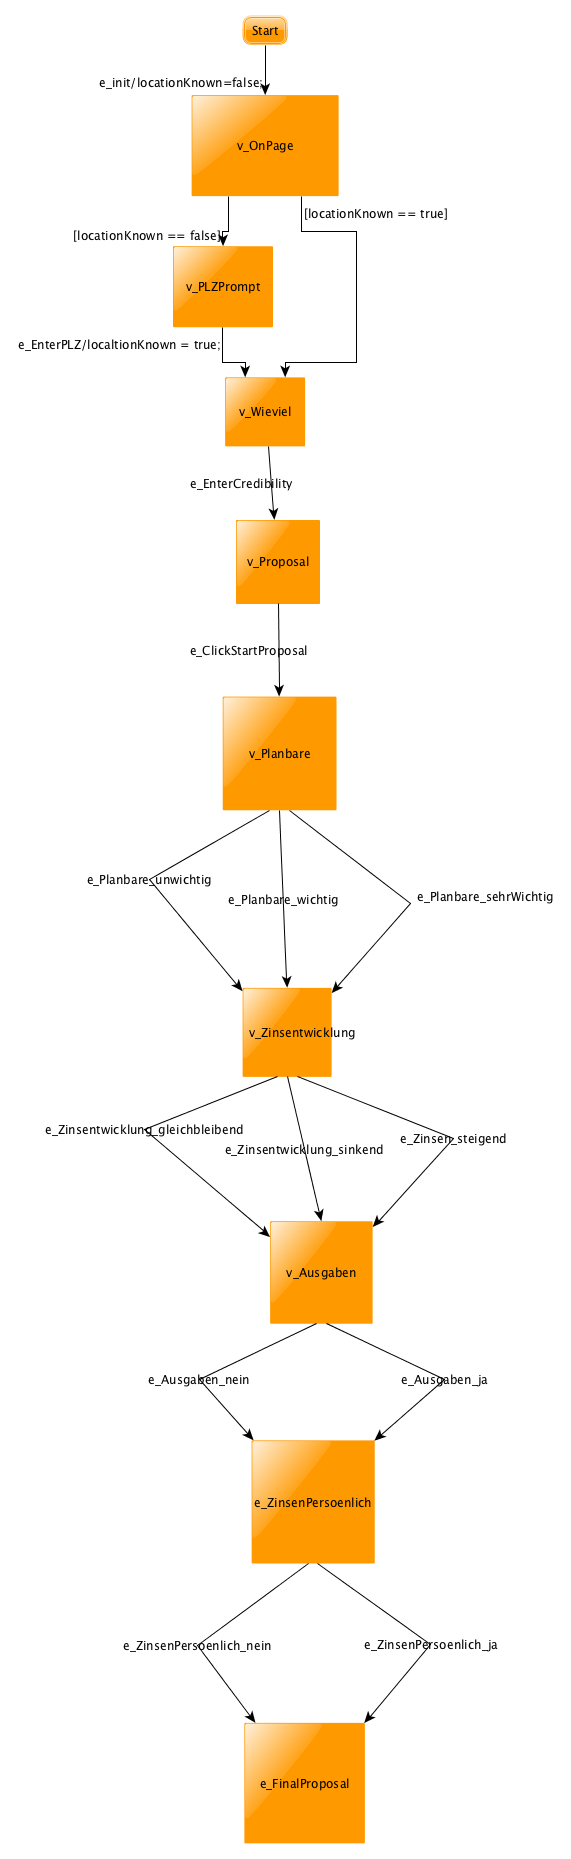
\includegraphics[width=1.0\textwidth]{figures/modell_abstract.png}
  \caption{}
  \label{fig:modell_abstract}
\end{figure}


\paragraph{Logik-Modellierung und Verfeinerung}


\begin{figure}[h] 
  \centering
     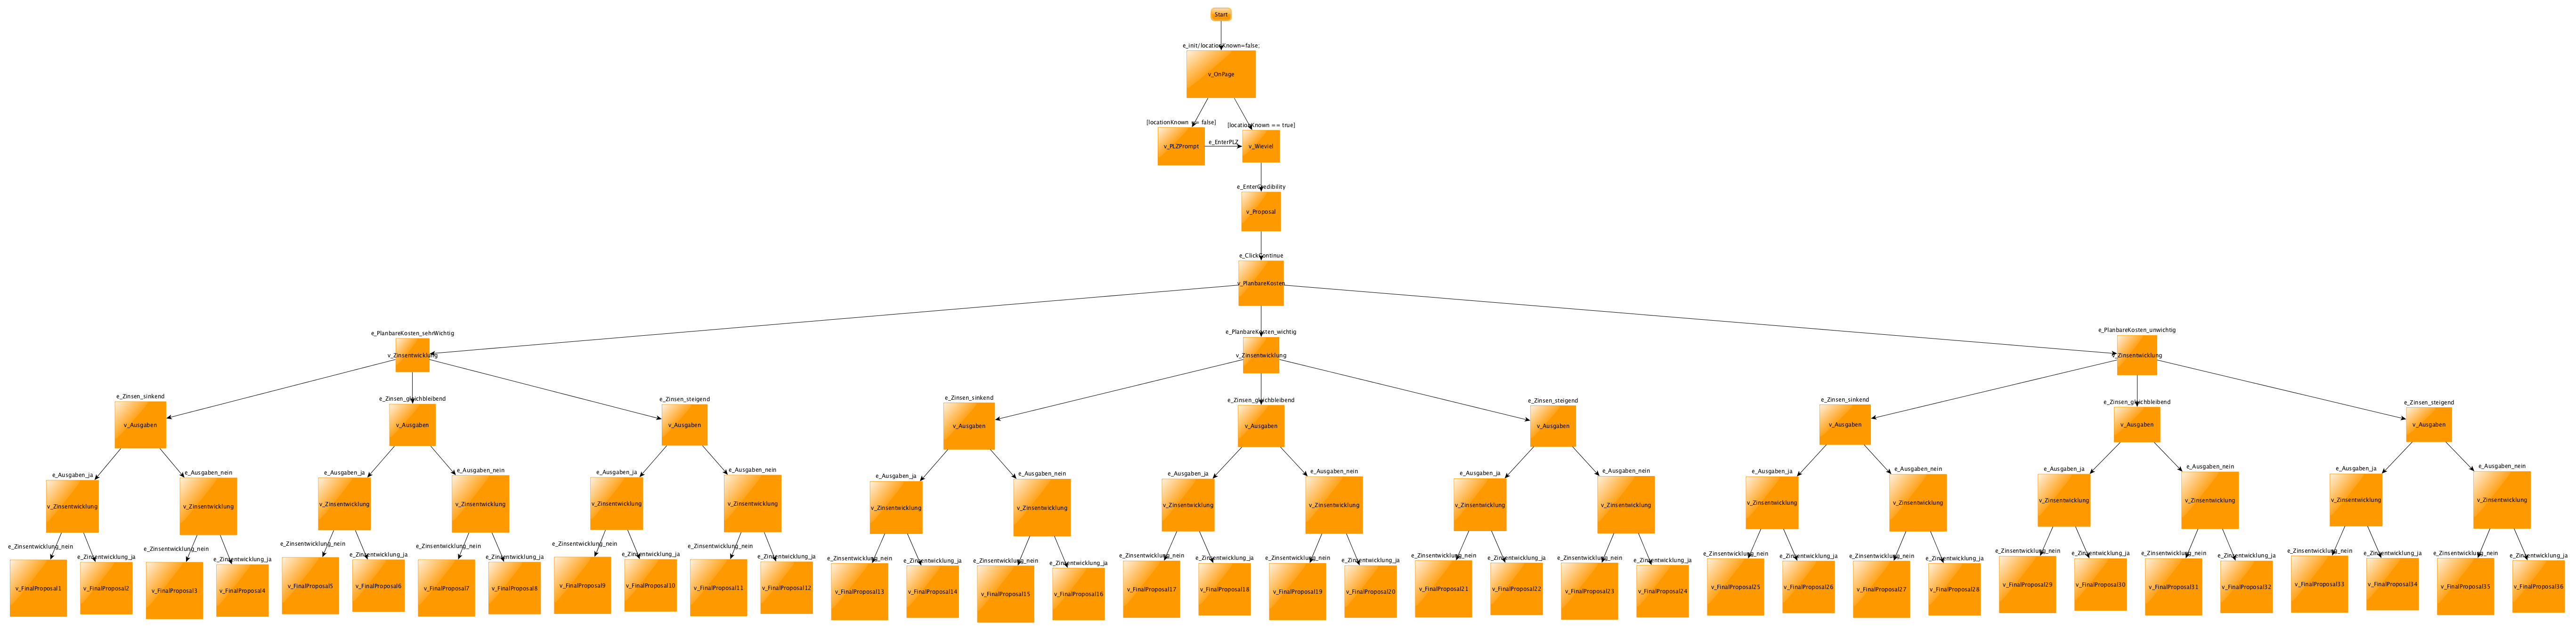
\includegraphics[width=1.5\textwidth, angle=90]{figures/modell_komplex.png}
  \caption{}
  \label{fig:modell_abstract}
\end{figure}


\begin{figure}[h] 
  \centering
     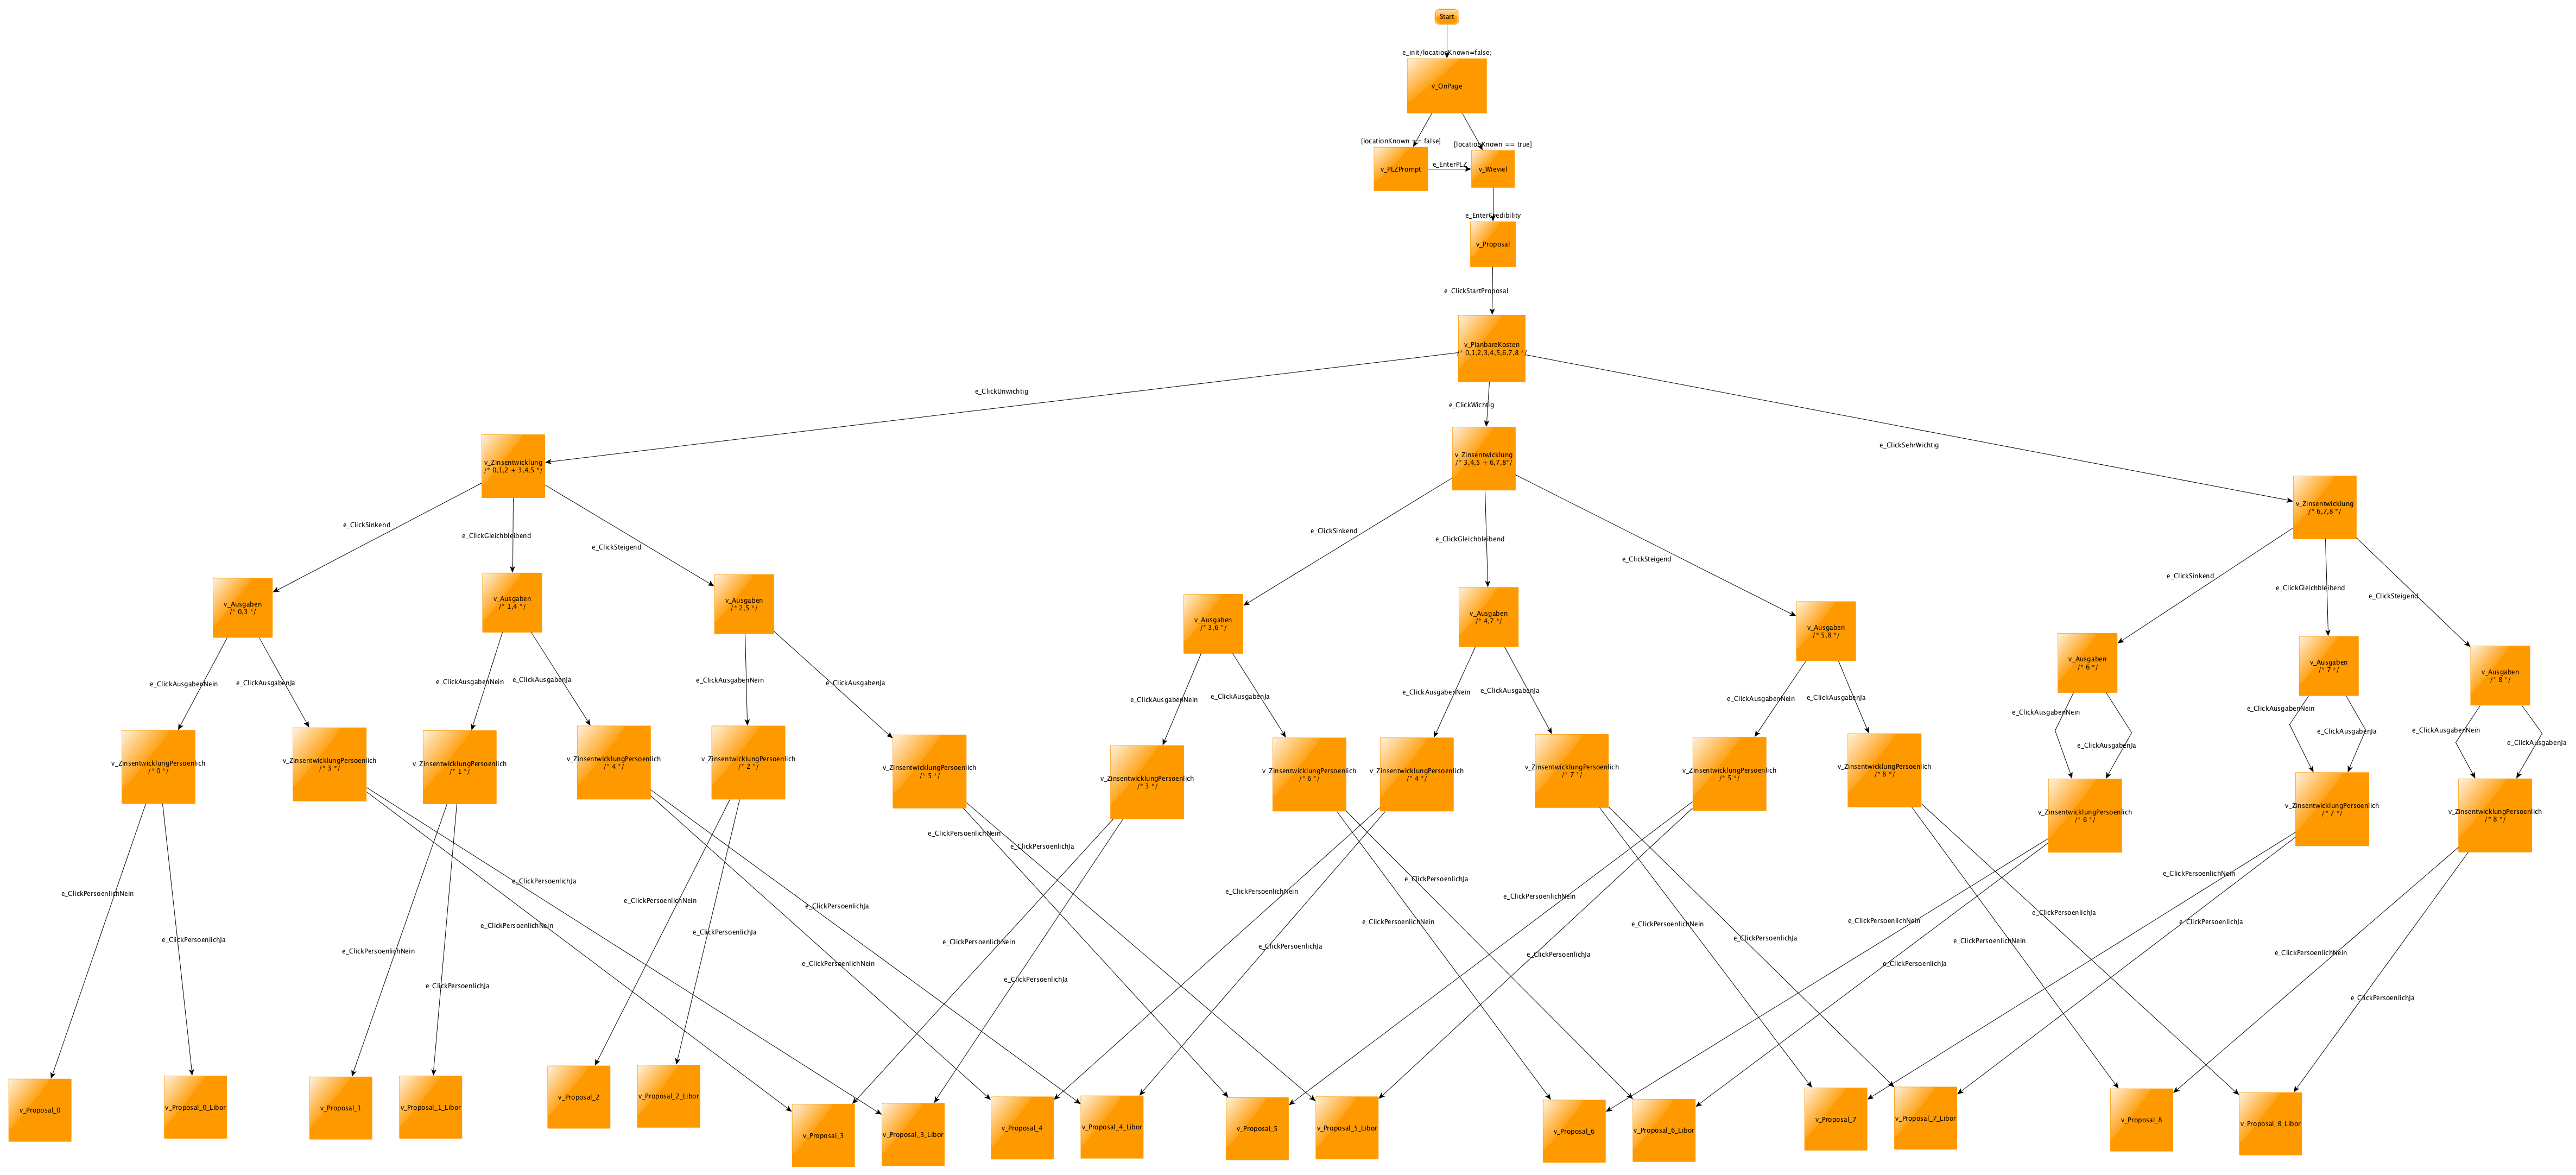
\includegraphics[width=1.5\textwidth, angle=90]{figures/modell_logisch.png}
  \caption{}
  \label{fig:modell_abstract}
\end{figure}

\section{Benefits}
...wie Robert Binder\cite{binder_model-based_2014} schon meinte: BDD decken oft nur kleine Teile des happy-path ab und geraten in Vergessenheit. Die Kombination mit MBT löst das Problem `nd, as a BDD specification and its associated test code base grows over time, work to maintain it either crowds out new development and testing or, typically, is simply ignored.'















\makeatletter\ifthesis@masterthesis
%%%%%%%%%%%%%%%%%%%%%%%%%%%%%%%%%%%%%%%%%%%%%%%%%%%%%%%%%%%%%%%%%%%%%%%%
\chapter{Diskussion \& Zusammenfassung}
\label{sec:discussion}
%%%%%%%%%%%%%%%%%%%%%%%%%%%%%%%%%%%%%%%%%%%%%%%%%%%%%%%%%%%%%%%%%%%%%%%%

\section{Vergleich mit verwandten Arbeiten}
\todo[color=yellow, inline]{@Boris, stark überarbeitet}
Im Laufe der Recherche für diese Arbeit hat sich gezeigt, dass modellbasiertes Testen ein sehr umfangreiches Thema ist. Es finden sich Arbeiten, Fallstudien und Anwendungsbeispiele in der Industrie, die zwar alle von modellbasiertem Testen sprechen, aber sich trotzdem gravierend unterscheiden. Deshalb ist ein Vergleich all dieser Methoden und Werkzeuge schwierig, unterstreicht aber gleichzeitig die Wichtigkeit von modellbasiertem Testen auf die Struktur des Projekts und die Art der zu testenden Software maßzuschneidern\todo{zu langer Satz}. Weiters kann \Gls{MBT} in allen bekannten Teststufen (siehe Abschnitt \ref{sec:teststufen} für eine Beschreibung der Stufen in der Domäne des Softwaretests) eingesetzt werden und abhängig von der Stärke\todo{anderes Wort} der bestehenden Testqualität macht es Sinn \Gls{MBT} nur punktuell einzusetzen. Mit dem in dieser Arbeit vorgeschlagenen Konzept ist dies, im Gegensatz zu gesamtheitlichen Lösungsansätzen für \Gls{MBT}, ohne weiteres möglich.\\
Viele Arbeiten wie \cite{pretschner_one_2005} \cite{pinheiro_model-based_2013} \cite{sensler_testautomatisierung_2011} präsentieren Konzepte und stellen die verwendeten Werkzeuge und das technische Vorgehen in den Mittelpunkt. Die menschliche Komponente wird dabei nicht erwähnt. In der Fallstudie dieser Arbeit hat sich gezeigt, dass es nicht reicht ein generisches aber technisch ausgereiftes Konzept einzuführen. In umfangreichen Softwareprojekten sind sehr viele Akteure mit den verschiedensten technischen und fachlichen Hintergründen beteiligt. Wenn die Teststrategie nicht diesen Umständen angepasst wird, leidet die Qualität des gesamten Projekts darunter. Ziel einer Teststrategie sollte sein, das Softwaretesten für so viele involvierte Parteien wie möglich verständlich zu machen. Im Sinne des gemeinsamen Vokabulars (die Grundprinzipien von \Gls{BDD} werden in Abschnitt \ref{sec:bdd} erklärt) ist es nur von Vorteil, wenn zwischen fachlichem und technischem Testen volle Transparenz herrscht. Weiters ist die Beteiligung der Akteure, die das zu entwickelnde Stück\todo{piece of Software :-) anderes Wort} Software spezifizieren, wünschenswert. Das Produktdesign\todo{Wieso nicht Qualität?} wird \textit{bewusster} und gleichzeitig präziser. Der zeitliche Aufwand für die Spezifikation erhöht sich möglicherweise, es wurde in der Vergangenheit mehrfach bewiesen, dass Ungenauigkeiten in der Spezifikation massive Auswirkungen auf das Endprodukt haben. Die Kosten zur Beseitigung erhöhen sich drastisch sich mit dem Fortschritt des Projekts. Deshalb ist der erhöhte Zeitaufwand für die Modellierung und Kommunikation in den frühen Stadien des Projekts gut investierte Zeit\todo{besser: wirkt sich positiv auf ... aus}.\\
Einige Werkzeuge\todo{Auflistung}, unter anderem auch das in den Experimenten von IBM \cite{farchi_using_2002} verwendete, setzen voraus, dass in den Modellen gewisse Abdeckungskriterien definiert werden müssen. Meist sind dies Werkzeuge, die textuelle Modellierungssprachen verwenden. Diese haben den Vorteil, dass sehr präzise Vor- und Nachbedingungen (Pre- und Postconditions) definiert werden können. Verglichen mit der Kombination von Graphwalker, mit grafischer Notation, und BDD-Tests sind diese weniger flexibel. Die Notation von Graphwalker ist so simpel gehalten, dass keinerlei Aussagen über Abdeckungs- oder Abbruchkriterien \todo{statt Stoppkriterien?} gemacht werden können. Das Modell und dessen Adapter-Code wird offline generiert (siehe Abschnitt \nameref{sec:online_offline} \ref{sec:online_offline}). Modell und Adaptercode\todo{Unterschiedliche Schreibweise, ganze Arbeit prüfen, besser ohne Bindestrich} können nun integriert oder von beliebiger Stelle aus gestartet werden. Das Modell und dessen Traversierung wird vollkommen entkoppelt. Das Modell muss also nicht dupliziert und modifiziert werden, um verschiedene Traversierungen zu generieren.\\
Grafische Notationen haben weiters den Vorteil, dass sie durch die Visualisierung leichter verständlich sind. Gleichzeitig besteht die Gefahr, dass Details übersehen werden oder gar nicht präzise genug notiert werden können. Das vorgestellte Konzept geht diesen Missstand auf zwei Arten an. Einerseits bietet das gewählte Werkzeuge eine sehr schlanke Syntax, die es nicht zulässt, dass wichtige Details unsichtbar modelliert werden können. Die grafische Syntax bestraft\todo{Wortwahl} den Testentwickler aber auch nicht, indem nur ein Subset von Fähigkeiten in der grafischen Syntax verfügbar gemacht werden. Andererseits, wird einfach auf BDD-Tests zurückgegeriffen wenn sehr spezifische Ein- und Ausgabe Kombinationen auf einem gewissen Zustand geprüft werden sollen. Wie in Abschnitt \ref{mbt_bdt} erklärt, kann durch die Vereinigung von \Gls{BDT} und \Gls{MBT} auf die Expressivität\todo{Wortwahl?} von \Gls{BDT} \textit{Then} Klauseln zurückgegriffen werden, wenn dies am nötigsten ist: In Knoten in denen Überprüfungen stattfinden, die in der grafischen Notation nicht ersichtlich sind.\\
Ein anderer Gesichtspunkt ist die Einfachheit der Einführung der Teststrategie. Generische Plattformen, wie die von \todo{citeauthor tag verwenden!}Zech et al. \cite{zech_generic_2012} vorgeschlagene, konzentrieren sich nicht nur auf die Modellierung und Traversierung des \Gls{SUT}. Vielmehr wollen sie eine gesamtheitliche Basis für das Testen schaffen. In großen Langzeitsoftwareprojekten ist eine solche Einführung aber extrem schwierig und in der Praxis selten. Die vorgeschlagene Teststrategie dieser Arbeit lässt eine inkrementelle und, zu agilen Projekten passende, iterative Einführung zu. Ebenso kann der modellbasierte Teil des Konzepts auf eigenständige Module des SUT's\todo{SUT ohne TAG!} beschränkt werden. Der BDD-Teil des Konzept kann zwar auch iterativ eingeführt werden, aber eine Beschränkung auf Teile des Projekts würde keinen Sinn machen. Dies hätte zur Folge, dass die Spezifikationen in Form von \Gls{COS} mittels zwei verschiedener System festgehalten oder versioniert werden müssten. Mittel- bis langfristig entstünden Überschneidungen und Unklarheiten, welche \Gls{COS} denn nun gültig sind und bei welchen es nötig ist, sie in das Regressionstesten einfließen zu lassen.\\
Robert Binders\todo{Citeauthor Tag!} Ansatz, den er in einer Präsentation \cite{binder_model-based_2014} erklärte aber in keiner schriftlichen Publikation detaillierte, scheint eine sehr ähnliche Idee zu verfolgen. Auch er hebt heraus wie sich \Gls{MBT} und \Gls{BDD} ergänzen und in die agile Vorgehensweise passen. Der Gedanke der gemeinsamen Verwendung von \Gls{BDT} und \Gls{MBT} wurde in dieser Arbeit weitergeführt. Daraus entstanden ist nicht nur die Empfehlung zur parallelen Verwendung beider Techniken, sondern auch eine Anleitung zur Vereinigung und Nutzung der jeweiligen Stärken.


\section{Kein Modellformat hat sich etabliert}
\label{sec:discussion_format}
Die Auswahl des Modellformats und die zugrunde liegende Notation ist eine fundamentale Entscheidung bei der Einführung von modellbasiertem Testen. Meist geht die Auswahl eines \Gls{MBT} Werkzeugs mit der Wahl des Modellformats einher. Die Ursprünge dieser Werkzeuge, für welche Art von Softwareprojekten diese zumeist eingesetzt wurden, sind unschwer an der unterstützten Modellnotation zu erkennen.  In der Praxis besteht eine Vielzahl von Notationen und Formaten, die auf sehr unterschiedlichen Prinzipien beruhen. Eine Transformation von einem Modellformat in ein anderes ist kaum möglich (beispielsweise lässt sich ein Modell in B Notation nur mit genauer Kenntnis des \Gls{SUT} in die Graphwalker-Notation konvertieren.)\\
Erschwerend kommt hinzu, dass gerade die großen kommerziellen Werkzeuge (wie Leiros Smartesting \footnote{Leiros Smartesting Produktseite \url{http://www.smartesting.com/en/}} oder Conformiq's \Gls{MBT} Toolsuite \footnote{Conformiq Produktseite \url{https://www.conformiq.com/products/}}) vollständig auf nicht-portable Eigenentwicklungen setzen. Diese Hersteller versuchen gezielt große Software-Projekte in ihr Ökosystem einzusperren, verpassen es aber die Branche der \Gls{MBT} Werkzeuge voranzutreiben. Sie vermarkten ihre Modellformate als Produktgeheimnis und verhindern dadurch die Entwicklung eines Standards der modellbasiertes Testen viel stärker in Erscheinung treten ließe. Weiters lassen sich Fähigkeiten der Werkzeuge kaum vergleichen. Während die Firma Conformiq ohne weiteres Testversionen ihrer vollständigen Toolsuite anbietet und die Open-Source Werkzeuge ohnehin frei evaluierbar sind, verlangt die Firma Leiros knapp 1000 Euro für eine akademische Lizenz. Auch auf Nachfrage des Autors wurde keine Demo- oder Testversion zum Zweck dieser Diplomarbeit zur Verfügung gestellt. Anhand offizieller Produktbeschreibungen und Quellen lässt sich nicht herausfinden wie sich der Workflow mit dem genannten Programm verhält, geschweige denn wie die zugrunde liegende Modellierung funktioniert.\\
Die Bemühungen der \Gls{OMG} mit dem UML Testing Profile eine einheitliche Sprache für modellbasiertes Testen zu schaffen ist ebenfalls nicht gelungen. Die Zahl der Publikationen die sich auf das UML Testing Profile stützen ist seit 2007 zwar konstant \footnote{Nach Recherche auf einschlägigen Portalen wie \url{http://ieeexplore.ieee.org/}}, trotzdem bietet kein dem Autor bekanntes Werkzeug Unterstützung dafür an. Zwar schlägt die offizielle Publikation der OMG\todo{TAG oder eintrag im Glossar} \cite{_model-driven_2007} manuelle Vorgehensweisen vor um UTP\todo{UTP Tag/Glossar} zu benutzen (siehe Kapitel \ref{sec:utp}), dies ist im Umfeld großer agiler Softwareprojekte aber nicht praktikabel. Zu viele Fehler könnten bei der manuellen Transformation von UTP-Diagramme\todo{UTP generell auf TAG prüfen} passieren.\\
Im Kontext von skriptbasierten GUI-Tests hat sich gezeigt, dass es mittel- bis langfristig enorme Vorteile mit sich bringt unabhängig von einem Hersteller zu bleiben. Diese Fallstudie war ebenfalls in der Finanzbranche angesiedelt \cite{graham_experiences_2012}. Die Fallstudie dieser Arbeit (siehe Abschnitt \ref{sec:fallstudie} \nameref{sec:fallstudie}) hat gezeigt, dass diese Erkenntnis auch im Umfeld des modellbasierten Testens gilt. Die Verwendung eines nicht-proprietären Modellformats bringt, abgesehen von der Flexibilität und Ungebundenheit, mehrere Vorteile:

\begin{itemize}
\item \textbf{Portabilität und Lesbarkeit:} Sollte ein Wechsel der Entwicklungsplattformen oder sogar der Teststrategie bevorstehen, können Modelle, die in einem offenen Format wie XML serialisiert werden können, mühelos transformiert werden. Es bleibt aber zu beachten, dass Transformationen zwischen fundamental verschiedenen Modellierparadigmen, trotz offener Serialisierung, kaum machbar sind.
\item \textbf{Wiederverwendbarkeit:} Leichtgewichtige und quelloffene Werkzeuge, wie Graphwalker\todo{verlinkung nur bei erster Erwähnung in dem Kapitel 5, also weiter oben!} (siehe Abschnitt \ref{sec:graphwalker}), erlauben die Weiterbenutzung bestehender skriptbasierter Tests. In der Praxis hat sich außerdem gezeigt, dass es sehr vorteilhaft ist Teile der Testbasis iterativ auf modellbasierte Tests zu übertragen. Der Aufbau der Modellierungskenntnisse im Team geschieht so breitflächiger und leichtgängiger, als wenn eine große Menge von Modellen und Adaptercode auf einmal erstellt werden müssen. Aus Sicht des Managements müssen weniger Aufwände initial riskiert werden, um projektrelevante Erfahrungen mit \Gls{MBT} zu sammeln. Aus Sicht der Entwickler besteht viel Freiraum in der Werkzeugauswahl für Adaptercode.
\item \textbf{Transparenz:} Technisch versierte Tester bzw. Testentwickler schätzen es, wenn das Parsen des Modells und die Testfallgenerierung möglichst transparent passieren. Bei omnipotenten \Gls{MBT} Lösungen ist dies nicht der Fall, da sie diese Details vor dem Benutzer verbergen wollen um attraktiv für die Fachbereiche zu wirken. In der Praxis sind aber Entwickler sowohl in der Auswahl des Werkzeugs als auch in der Erstellung der Modelle stark beteiligt.
\end{itemize}


% \section{Erweiterung des Begriffs `Test Non-Stop'}
% Nicht nur End to End Tests sondern Testen in Produktion\\
% Erstens: Ansatz von Google mit Machine Learning Ansätze

% \section{Priorisierung und Erweiterung von Unit-Tests}
% \label{sec:discussion_unit}
% Unit-Tests müssen noch mehr an Wichtigkeit gewinnen im agilen Umfeld \cite{linz_testing_2014}, auch Google Testing Blog zitieren. Ich schlage eine noch extremere Test-Pyramide vor (unproportional GUTE Unit-Tests, basierend auf MBT).\\
% Sogar GUI Tests können als Unit-Test angesehen werden, mocken von Daten und Umgebungen --> Verweis zu Service-Virtualisierungen in großen Tools wie HP UFT\\
% Klarstellen, dass End2End Systemtests extrem zeitraubende Unterfangen sind aber gleichzeitig sehr schnell gebrochen werden können (durch Technologieänderungen, Umstellungen der GUU/Plattform usw).

%%%%%%%%%%%%%%%%%%%%%%%%%%%%%%%%%%%%%%%%%%%%%%%%%%%%
\section{Zusammenfassung und Ausblick}
\label{sec:conclusion}
%%%%%%%%%%%%%%%%%%%%%%%%%%%%%%%%%%%%%%%%%%%%%%%%%%%%%%%%%%%%%%%%%%%%%%%%
Die Komplexität moderner Softwaresysteme ist bereits sehr hoch und wird mit wachsender Rechenleistung und Konnektivität noch höher. Es braucht Strategien, um der steigenden Komplexität in der Qualitätssicherung gerecht zu werden. Das Feld der modellbasierten Testtechnologien ist vielfältig. Diese Arbeit zeigt, dass \Gls{MBT} automatische Tests weiter stärken kann, nicht nur um wiederkehrende und sich wiederholende Tätigkeiten zu testen. Auch die vollständige Exploration der Programmzweige und die damit verbundene Gewissheit ermöglicht \Gls{MBT} so einfach wie keine andere Testmethodik.\\
Im Kapitel \ref{sec:problemdescription} \nameref{sec:problemdescription} wurden \Gls{MBT} Werkzeuge für den Einsatz auf Ebene des Komponententests und des Integrationstests erprobt. Das Werkzeug \textit{ModelJUnit} ist in der Verwendung an die weit verbreiteten Komponententestwerkzeuge angelehnt. Modelle werden als Java-Klasse dargestellt und Zustandsübergänge werden auf Methodenebene annotiert. Das Werkzeug bietet keine grafische Notation und erzeugt auch keine visuelle Darstellung. Die Stärken von ModelJUnit liegen in der Einfachheit und in der guten Integrierbarkeit in bestehende Strukturen. Nachteilig wirkt sich aus, dass die Modelle weder die Verständlichkeit von grafischen Modellen, noch die Ausdrucksstärke von textuellen Notationen besitzt.\\
Auf Integrationstestebene gab es Bemühungen, den bekannten UML-Standard auszubauen und für die Definition von Testmodellen verwenden zu können. Das Ergebnis ist das UML Testing Profile. Dabei wurde die Sprache UML durch das Konzept der Profile erweitert und bietet nun Notationsmöglichkeiten speziell für das Testen. UTP\todo{UTP ohne TAG, check des ganzen discussion.tex file!} bietet zwar einige essentielle Konzepte, die für den Gebrauch in komplexen Softwareprojekten nötig sind, aber wie die Generierung der Modelle erfolgen soll, bleibt den Werkzeugentwicklern vorbehalten. Eine Möglichkeit ist das manuelle Mapping von UTP Elementen zu JUnit, wie in Kapitel \ref{sec:utp} beschrieben. Dies gestaltet sich allerdings als recht aufwendig und bietet wenig zusätzlichen Nutzen, verglichen mit der direkten Erstellung der JUnit Testfälle ohne den Umweg über UTP.\\
Auch das in Kapitel \ref{sec:graphwalker} beschriebene Werkzeug \textit{Graphwalker} lässt sich auf Integrationstestebene einsetzen. Es bietet einen Parser, der das Einlesen von Modellen in Form von Graphen ermöglicht. Graphwalker generiert daraus Java-Code, der mit Code für die Verbindung zum \Gls{SUT} gefüllt werden muss. Schlussendlich traviersiert Graphwalker das Modell auf die gewünschte Art und Weise. Das Werkzeug befähigt den Tester modellbasierte Tests gegen das \Gls{SUT} auszuführen, ohne auf gewohnte Mittel zur Verbindungsherstellung mit dem \Gls{SUT} verzichten zu müssen. Schnittstellentests könnten beispielsweise weiterhin mit \textit{SoapUI}, Oberflächentests mit \textit{Selenium} realisiert werden.\\
Die Fallstudie \ref{sec:fallstudie} \nameref{sec:fallstudie} hat gezeigt, dass modellbasierte Tests sinnvoll in agilen Softwareprojekten eingesetzt werden können, auch ohne damit andere Testmethodiken zu verdrängen. Sogar eine schrittweise Einführung in ein großes bestehendes Softwareprojekt ist möglich, vorausgesetzt es werden flexible Werkzeuge genutzt. Der Einsatz von Graphwalker hat sich als sehr unkompliziert herausgestellt, weil wenige tiefgreifende Eingriffe in die bestehende Teststrategie gemacht werden müssen. Das Werkzeug kann unabhängig von der gegebenen Umgebung genutzt werden. Es integriert sich, wenn gewünscht, auch in große Testmanagementprogramme von HP oder IBM. Dies ist durch die offene Java Schnittstelle möglich, die Graphwalker mitbringt. Außerdem ist es nicht nötig bestehenden Adapter-Code neu zu schreiben. Testfälle die als Java-Code vorliegen (z.B. Selenium) oder zumindest durch eine Java Schnittstelle ansprechbar sind (z.B. SoapUI) können in Graphwalker Tests eingebunden werden, weil Graphwalker selbst keine Annahme über das Ansprechen des \Gls{SUT} trifft.\\
%Schreiben wie die Kombination von BDD den Fachbereich einbindet und seine punktuellen Eigenschaften verliert
Das Resultatskapitel \ref{sec:results} hat eine Teststrategie vorgestellt, die auf die Schwächen bestehender Lösungen eingeht. Mittels der durchdachten Orchestrierung mehrerer Testansätze (gewöhnliche Komponententests, \Gls{BDT} und \Gls{MBT}) kann hocheffiziente Qualitätssicherung realisiert werden. Durch die Nutzung einer gemeinsamen Basis für Adapter-Code (der Testing-API, siehe Abschnitt \ref{sec:testing_api}) kann kurzfristig Wartungsaufwand minimiert werden und langfristig Zukunftssicherheit bei einem Werkzeugwechsel geboten werden. 
Abhängig vom fachlichen Kontext, können aufbauend darauf \Gls{BDT} und \Gls{MBT} Tests parallel zueinander eingesetzt werden. Beide Methodiken können dort verwendet werden, wo sie am besten passen, ohne damit den Wartungsaufwand zu erhöhen, weil sie beide von einer gemeinsamen Schicht konsumieren\todo{formulierung konsumieren}.\\

Es hat sich außerdem gezeigt, dass eine Verschmelzung von \Gls{BDT} und \Gls{MBT} sinnvoll sein kann. Die Techniken haben strukturelle Ähnlichkeiten, wenn man betrachtet wie Tests definiert werden und welche Sicht auf das \Gls{SUT} sie einnehmen. \Gls{BDT} definiert mit seinen \textit{Given} und \textit{When} Teilen eine Aktion, die auf einem System in einem bestimmten Zustand ausgeführt wird. Der \textit{Then} Teil ist eine Aneinanderreihung von Überprüfungen, die zusammen evaluiert und über das Resultat des Testfalls entscheiden. Sieht man das \Gls{SUT} als abstrahierten endlichen Automaten und visualisiert man einen solchen \textit{Given-When-Then} Block, dann ist ein \Gls{BDT} Test ein Pfad von einem Knoten zu einem anderen. Sowohl die beiden Notationen, als auch die darunterliegenden Technologien haben ihre Stärken und Schwächen. Der \textit{Given} Teil ist eine kurze Zusammenfassung des Systemzustandes und kann als Modell genauer ausgedrückt werden. Wenn der Zustand aus dem Kontext klar ist, kann es aber genauso valide sein den knappen Einzeiler des \textit{Given} Teil zu verwenden und mit nur einem Knoten im Modell zu starten, der diesen repräsentiert. Der \textit{When} Teil kann fälschlicherweise suggerieren, dass eine Aktion eine atomare Handlung ist oder keine Alternativpfade zum Endzustand bestehen. In einem Modell kann durch mehrere Äste ausgeführt werden, auf welche Arten der Endzustand erreicht werden kann. Auf der Benutzeroberfläche wäre beispielsweise denkbar, dass eine Maske über einen Button, ein Kontextmenü oder ein Tastaturkürzel erreicht werden kann. Zuletzt steht der \textit{Then} Teil, der sich in einem Modell nicht von anderen Knoten unterscheidet. In der Realität finden dort aber die wichtigsten Überprüfungen statt. Diese verbergen sich im Code und sind auf grafischer Ebene nicht sichtbar. Viel ausdrücklicher ist hier \Gls{BDT} indem die Erfolgsbedingungen klar ausformuliert werden. Eine Ebene über einzelnen Tests können auch \Gls{BDT}-Szenarien als Modell dargestellt werden und wiederum mit den ausdrucksstarken \textit{Then}\todo{Vorsicht Schreibweise, alle mit Anfangsbuchstaben groß (Kontrolle Arbeit!)} Statements beendet werden.\\


Für die weitere Festigung dieses Themengebiets wären mehrjährige Fallstudien großer und lange andauernder Softwareprojekte höchst interessant. Durch den Vergleich von Qualitätsmetriken, aufgenommen während modellbasierte und nicht-modellbasierte Werkzeuge im Einsatz waren, ließen sich Schlüsse auf die tatsächliche Produktivitäts- und Qualitätssteigerung schließen die \Gls{MBT} verspricht.\\
Weiters bedarf es einer gewissen Standardisierung von Modellformaten und Werkzeugschnittstellen (siehe die Diskussion in Abschnitt \ref{sec:discussion_format}). Gegenwärtig werden Unternehmen eher abgeschreckt, Ressourcen in eine modellbasierte Strategie zu investieren für die keine entsprechende Standardisierung der Sprache vorliegt. Mit dem Einstellen\todo{Formulierung, verstehe nicht ganz was Du damit meinst} eines kritischen Werkzeugs könnten langjährige Bemühungen auf einen Schlag obsolet werden. Dieser Umstand kann durch die Möglichkeit Testartefakten mühelos wiederverwenden zu können, gemildert werden. Das wiederum ist zur Zeit nicht möglich, da die vielen erhältlichen Werkzeuge grundlegend verschiedene Ansätze verfolgen.




























%%%%%%%%%%%%%%%%%%%%%%%%%%%%%%%%%%%%%%%%%%%%%%%%%%%%%%%%%%%%%%%%%%%%%%%%
\chapter{Zusammenfassung und Ausblick}
\label{sec:conclusion}
%%%%%%%%%%%%%%%%%%%%%%%%%%%%%%%%%%%%%%%%%%%%%%%%%%%%%%%%%%%%%%%%%%%%%%%%

\makeatletter\ifthesis@masterthesis
Die Zusammenfassung ist nach der Kurzfassung der am häufigsten gelesene Teil, da viele Leser aus Zeitknappheit Arbeiten im Schnellverfahren konsumieren und rasch zur Zusammenfassung blättern. Hier hat man die Chance, dem Leser noch einmal die zentralen Ideen und Ergebnisse der Diplomarbeit zu vermitteln.

Im Gegensatz zur Kurzfassung sind die Leser mit der Problemstellung und der Terminologie bereits vertraut. In der Länge hat man deutlich mehr Spielraum als bei der Kurzfassung, die Zusammenfassung sollte inklusive Ausblick 2 bis max. 10 Seiten umfassen. Hier sollten kompakt die Antworten auf die in der Zielsetzung aufgeworfenen Fragen (Hypothesen) gegeben werden.

Neben einer Zusammenfassung der wichtigsten Ergebnisse sollte auch ein Ausblick gegeben werden: Aufzeigen des Bedarfs an zukünftiger Forschung, potentielle Anwendungsmöglichkeiten der vorgestellten Lösung etc.

In Summe sollte die Zusammenfassung dem Leser die wissenschaftliche und, wenn vorhanden, praktische Relevanz der Arbeit klar und verständlich darlegen.
\fi\makeatother

\chapter{Hinweise zur Literatur}
\label{sec:references}

\section{Literatursuche}

Der Vollzugang zu einigen Publikationen ist nur intern aus dem TU-Netz möglich. Um auf möglichst viele Papers extern zugreifen zu können, wird von der TU Wien eine \href{http://www.zid.tuwien.ac.at/tunet/vpn/extern/}{VPN-Zugangsmöglichkeit} angeboten, diesen VPN-Zugang bitte gleich einrichten.

Besonders ergiebig sind folgende Search-Engines:\\
\href{http://academic.research.microsoft.com/}{Microsoft Academic}\\
\href{http://dl.acm.org/}{ACM-Datenbank}\\
\href{http://scholar.google.com/}{Google Scholar}

Wir empfehlen, vor Beginn Ihrer Arbeit einige Diplomarbeiten, die am INSO oder generell an der Fakultät für Informatik verfaßt wurden, zu Ihrem Themenbereich zu suchen und Aufbau, Schreibstil, Art der Abbildungen etc. durchzuschauen. Arbeiten finden Sie \href{http://media.obvsg.at/tuw?query=grechenig&metaname=swishdefault&submit=Suche+starten&sbm=tuw*&lbm=*&lbc=*&searchtype=sim&.cgifields=metaname}{hier}.

Weitere Datenbanken und Suchmaschinen:\\
\href{http://rzblx1.uni-regensburg.de/ezeit/search.phtml?bibid=UBTUW&colors=7&lang=de}{Elektronische Zeitschriftenbibliothek der TU Wien}\\
\href{http://citeseer.ist.psu.edu/index;jsessionid=BF9BD5A89D42210F60E5CA88B40BAD9C}{Scientific Literature Digital Library (CiteSeer)}\\
\href{http://www.ingentaconnect.com/}{Ingenta}\\
\href{http://www.theiet.org/resources/inspec/}{INSPEC}

Journals:\\
\href{http://ieeexplore.ieee.org/}{IEEE - Institute of Electrical and Electronics Engineers, Inc. - Library}\\
\href{http://www.springerlink.com/?MUD=MP}{Verlag Springer - Springer Link}\\
\href{http://www.elsevier.com/wps/find/homepage.cws_home}{Elsevier}

Bibliotheken und Online-Kataloge:\\
\href{http://search.obvsg.at/primo_library/libweb/action/search.do?vid=ACC}{Online-Kataloge des Österreichischen Bibliothekenverbundes}\\
\href{http://aleph.ub.tuwien.ac.at/}{Online-Katalog der TU Wien} (ALEPH)\\
\href{http://www.informatik.uni-trier.de/}{Digital Bibliography \& Library Project (DBLP) of University of Trier}\\
\href{http://liinwww.ira.uka.de/bibliography/}{The Collection of Computer Science Bibliographies}

\section{BibLatex}

Biblatex beitet verschiedene Möglichkeiten an um Literatur zu referenzieren. Die beiden häufigsten Befehle sind \verb|\cite| und \verb|\citeauthor|.

Beispiele wie referenziert werden kann:\\
\citeauthor{fankhauser:2009:softwaretechnik-security} beschreiben in \cite{fankhauser:2009:softwaretechnik-security} \dots\\
In \cite{schanes:2011:voip-fuzzer} zeigt \citeauthor{schanes:2011:voip-fuzzer} wie \dots
Weitere Informationen können von \cite{oasis:2010:homepage} in \cite{oasis:2010:homepage} entnommen werden.

Wir empfehlen JabRef um die Literaturdatenbank zu verwalten.
\chapter{Algorithmen und Quellcode}

\section{Beispiele für Quellcode}

Beispiel eines Quellcodes ist im Quellcode \ref{lst:shortcode} zu finden.

\begin{lstlisting}[caption={Short code},label=lst:shortcode]
//Start Program
System.out.println("Hello World!");
//End Program
\end{lstlisting}


\section{Beispiele für Algorithmen}

Algorithmus \ref{alg:samplealgorithm} dient als Beispiel.

\begin{algorithm}[t]
\SetKwData{Left}{left}
\SetKwData{This}{this}
\SetKwData{Up}{up}
\SetKwFunction{Union}{Union}
\SetKwFunction{FindCompress}{FindCompress}
\SetKwInOut{Input}{input}
\SetKwInOut{Output}{output}

\Input{A bitmap $Im$ of size $w\times l$}
\Output{A partition of the bitmap}

\BlankLine

\emph{special treatment of the first line}\;
\For{$i\leftarrow 2$ \KwTo $l$}{
\emph{special treatment of the first element of line $i$}\;
\For{$j\leftarrow 2$ \KwTo $w$}{\label{forins}
\Left$\leftarrow$ \FindCompress{$Im[i,j-1]$}\;
\Up$\leftarrow$ \FindCompress{$Im[i-1,]$}\;
\This$\leftarrow$ \FindCompress{$Im[i,j]$}\;
\If(\tcp*[r]{O(\Left,\This)==1}){\Left compatible with \This}{\label{lt}
\lIf{\Left $<$ \This}{\Union{\Left,\This}}\;
\lElse{\Union{\This,\Left}\;}
}
\If(\tcp*[r]{O(\Up,\This)==1}){\Up compatible with \This}{\label{ut}
\lIf{\Up $<$ \This}{\Union{\Up,\This}}\;
\tcp{\This is put under \Up to keep tree as flat as possible}\label{cmt}
\lElse{\Union{\This,\Up}}\tcp*[r]{\This linked to \Up}\label{lelse}
}
}
\lForEach{element $e$ of the line $i$}{\FindCompress{p}}
}
\caption{Sample algorithm}\label{alg:samplealgorithm}
\end{algorithm}


% insert bibliography and such stuff
\BackMatter

\cleardoublepage
\appendix

%%%%%%%%%%%%%%%%%%%%%%%%%%%%%%%%%%%%%%%%%%%%%%%%%%%%%%%%%%%%%%%%%%%%%%%%
\chapter{\appendixlabel}
%%%%%%%%%%%%%%%%%%%%%%%%%%%%%%%%%%%%%%%%%%%%%%%%%%%%%%%%%%%%%%%%%%%%%%%%
\section{Interview Leitfaden}
\label{app:leitfaden}
Als Grundlage zur Konzeption der in Kapitel \ref{sec:results} beschriebenen Teststrategie wurden Interviews mit dem leitenden Architekten der Applikation, einem Entwickler, einer Business-Analystin und einem Testverantwortlichen geführt. Das Dokument in Abbildung \ref{fig:leitfaden} diente dabei als Leitfaden.

\begin{figure}[h] 
  \centering
     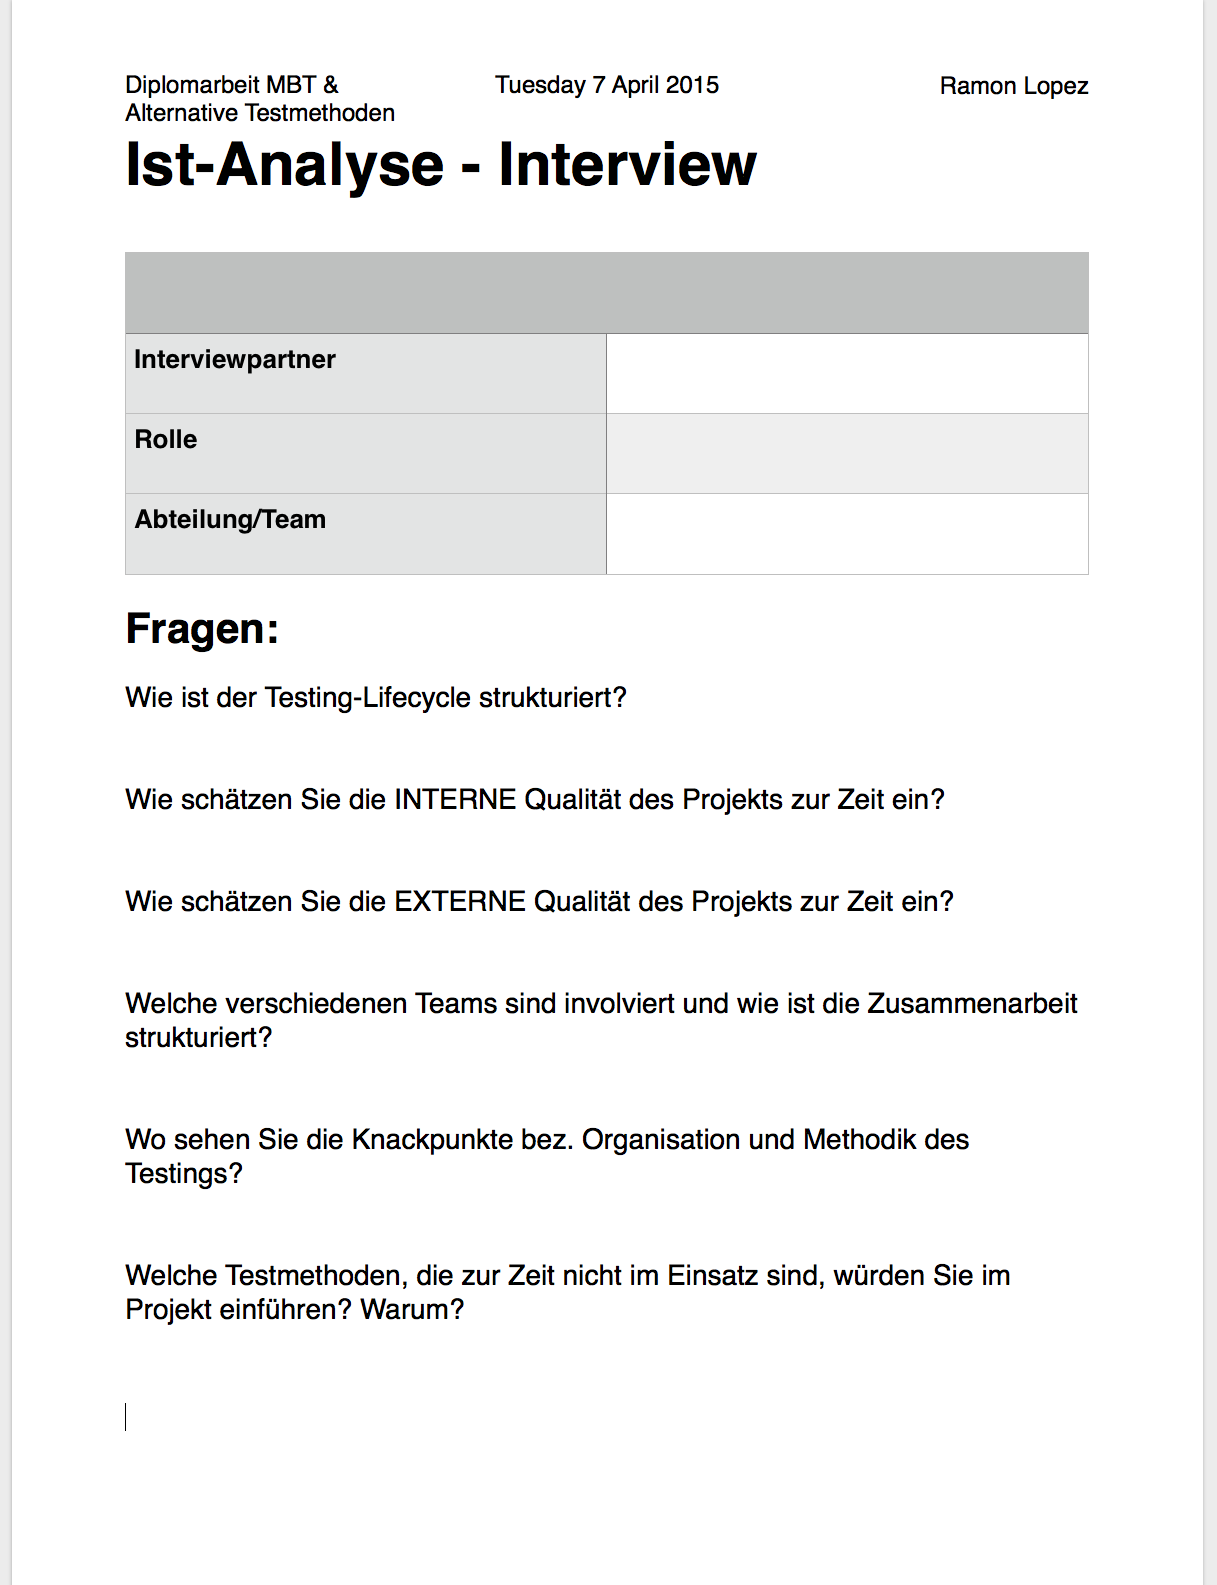
\includegraphics[width=1.0\textwidth]{figures/leitfaden.png}
  \caption{Interview Leitfadendokument}
  \label{fig:leitfaden}
\end{figure}

\section{SoapUI Testfallaufruf aus Graphwalker}
\label{app:soap}
Das folgende Beispiel \ref{code:soap_graphwalker} zeigt wie in einem Graphwalker Testfall SoapUI als Adapter-Code verwendet werden kann.\\
Die drei Methoden zum Schluss zeigen verschiedene Möglichkeiten wie Graphwalker das Testmodell traversieren kann.\\
Das vollständige Beispiel (inklusive einer vorgetäuschten REST-Schnittstelle, die der SoapUI Testfall anspricht) ist zu finden unter: \url{https://github.com/SH4DY/graphwalker-soapui/}


\begin{lstlisting}[language=Java,caption=SimpleTest.java, label=code:soap_graphwalker]
package org.myorg.testautomation;

import com.eviware.soapui.tools.SoapUITestCaseRunner;
import org.graphwalker.core.condition.EdgeCoverage;
import org.graphwalker.core.condition.ReachedVertex;
import org.graphwalker.core.condition.TimeDuration;
import org.graphwalker.core.generator.AStarPath;
import org.graphwalker.core.generator.RandomPath;
import org.graphwalker.core.machine.ExecutionContext;
import org.graphwalker.java.test.TestBuilder;
import org.junit.Test;

import java.nio.file.Path;
import java.nio.file.Paths;
import java.util.concurrent.TimeUnit;

/**
 * SoapUI 5 project running on Graphwalker
 *
 * This class represents the operations to be executed
 * when Graphwalker traverses the model. The stub generated
 * by the Graphwalker CLI is in the target directory.
 *
 * Methods prefixed with "e_" are edges, "v_" are vertices.
 *
 * The underlying model can be found at {@link SimpleTest#MODEL_PATH}
 *
 * The underlying model can be found at {@link SimpleTest#SOAPUI_PROJECT_PATH}
 * Methods in this class call according testsuites in the given project
 */
public class SimpleTest extends ExecutionContext implements Login {
    public static final Path MODEL_PATH = Paths.get("org/myorg/testautomation/Login.graphml");
    public static final String SOAPUI_PROJECT_PATH = "login/src/main/resources/soapui/GW-Test-Project-soapui-project.xml";

    @Override
    public void e_InvalidCredentials() {

        //Try login with invalid credentials
        SoapUITestCaseRunner runner = new SoapUITestCaseRunner();
        runner.setProjectFile(SOAPUI_PROJECT_PATH);
        runner.setTestSuite("InvalidLogin");
        try {
            runner.run();
        } catch (Exception e) {
            e.printStackTrace();
        }
    }

    @Override
    public void e_ValidCredentials() {

        //Invoke SoapUI testcase with valid credentials
        SoapUITestCaseRunner runner = new SoapUITestCaseRunner();
        runner.setProjectFile(SOAPUI_PROJECT_PATH);
        runner.setTestSuite("ValidLogin");
        try {
            runner.run();
        } catch (Exception e) {
            e.printStackTrace();
        }
    }

    //All the other edges and nodes have to be overriden as well

    @Test
    public void runSmokeTest() {
        new TestBuilder()
                .setModel(MODEL_PATH)
                .setContext(new SimpleTest())
                .setPathGenerator(new AStarPath(new ReachedVertex("v_Browse")))
                .setStart("e_Init")
                .execute();
    }

    @Test
    public void runFunctionalTest() {
        new TestBuilder()
                .setModel(MODEL_PATH)
                .setContext(new SimpleTest())
                .setPathGenerator(new RandomPath(new EdgeCoverage(100)))
                .setStart("e_Init")
                .execute();
    }

    //@Test
    public void runStabilityTest() {
        new TestBuilder()
                .setModel(MODEL_PATH)
                .setContext(new SimpleTest())
                .setPathGenerator(new RandomPath(new TimeDuration(30, TimeUnit.SECONDS)))
                .setStart("e_Init")
                .execute();
    }

}
\end{lstlisting}


\section{Graphwalker Testsuite am Beispiel Hypothekarrechner mit Selenium}
Es folgt der Code zum Beispiel aus Kapitel \ref{sec:results} - \Newnameref{sec:results}. Hier wird das \Gls{SUT} im GraphML Format dargestellt. Graphwalker erzeugt ein Java Interface, welches der Testentwickler mit Adapter-Code befüllt. In diesem Beispiel wurde Selenium verwendet um die Applikation anzusteuern.\\

Das Codebeispiel \ref{code:gw_generated} zeigt das von Graphwalker generierte Java Interface. Wie das zugrundeliegende Modell \ref{fig:modell_logisch} erstellt wurde, wird im Abschnitt \ref{sec:results_modellierung} beschrieben.\\

Im Listing \ref{code:gw_selenium} wird das generierte Interface implementiert. Nicht alle Knoten und Kanten müssen Adapter-Code enthalten.\\

Das vollständige Beispiel, inklusive der generierten GraphML Dateien, ist zu finden unter: \url{https://github.com/SH4DY/ImexTest/}

\begin{lstlisting}[language=Java,caption=ImexTest.java, label=code:gw_selenium]
package com.shady.imextest.modelimplementations;

import com.shady.imextest.ModellLogisch;
import org.graphwalker.core.condition.EdgeCoverage;
import org.graphwalker.core.condition.ReachedVertex;
import org.graphwalker.core.generator.AStarPath;
import org.graphwalker.core.generator.RandomPath;
import org.graphwalker.core.machine.ExecutionContext;
import org.graphwalker.java.annotation.GraphWalker;
import org.graphwalker.java.test.Result;
import org.graphwalker.java.test.TestBuilder;
import org.junit.Assert;
import org.junit.Test;
import org.openqa.selenium.*;
import org.openqa.selenium.chrome.ChromeDriver;
import org.openqa.selenium.support.ui.*;

import java.nio.file.Path;
import java.nio.file.Paths;
import java.util.concurrent.TimeUnit;

/**
 * Diese Klasse beinhaltet alle Kanten und Knoten aus dem entsprechenden logischen Modell des
 * Hypothekarrechners. Im Modell sind es 51 Knoten und 66 Kanten. Im Code sind es aber deutlich
 * weniger Methoden.
 *
 */
@GraphWalker(value = "random(edge_coverage(100))", start = "e_init")
public class ImexTest extends ExecutionContext implements ModellLogisch {

    private final static Path MODEL_PATH = Paths.get("com/shady/imextest/ModellLogisch.graphml");
    private WebDriver driver;

    private final String HYPO_URL= "https://www.raiffeisen.ch/rch/de/privatkunden/hypotheken/wohneigentum-kaufen/wieviel-eigenheim-kann-ich-mir-leisten.html";

//    @Test
//    public void runSmokeTest() {
//        TestBuilder tb = new TestBuilder()
//                .addModel(MODEL_PATH,
//                        new ImexTest().setPathGenerator(new AStarPath(new ReachedVertex("v_Proposal_7_Libor"))));
//
//        Result result = tb.execute();
//        System.out.println("Done: [" + result.getErrors().toString() + "," + result.getFailedCount() + "]");
//    }

    @Test
    public void runFunctionalTest() {
                TestBuilder tb = new TestBuilder()
                        .addModel(MODEL_PATH,
                                new ImexTest().setPathGenerator(new RandomPath(new EdgeCoverage(100))));
        Result result = tb.execute();
        System.out.println("Done: [" + result.getErrors().toString() + "," + result.getFailedCount() + "]");

    }
//
//    @Test
//    public void runStabilityTest() {
//        new TestBuilder()
//                .setModel(MODEL_PATH)
//                .setContext(new ImexTest())
//                .setPathGenerator(new RandomPath(new TimeDuration(30, TimeUnit.SECONDS)))
//                .setStart("e_Init")
//                .execute();
//    }

    @Override
    public void e_init() {
        driver = new ChromeDriver();

        //Selenium wartet somit 10 Sek. bevor eine NotFound exception geworfen wird.
        driver.manage().timeouts().implicitlyWait(10, TimeUnit.SECONDS);
    }


    @Override
    public void v_OnPage() {
        driver.get(HYPO_URL);
    }


    @Override
    public void v_PLZPrompt() {
    }

    @Override
    public void e_EnterPLZ() {
        WebElement searchBox = driver.findElement(By.className("dropdown-toggle"));
        searchBox.sendKeys("6900");

        WebDriverWait wait = new WebDriverWait(driver, 10);
        wait.until(ExpectedConditions.elementToBeClickable(By.partialLinkText("Lugano")));

        driver.findElement(By.partialLinkText("Lugano")).click();

    }

    @Override
    public void v_Wieviel() {
    }

    @Override
    public void e_EnterCredibility() {

        Wait wait = new FluentWait<WebDriver>(driver)
                .withTimeout(5, TimeUnit.SECONDS)
                .pollingEvery(500, TimeUnit.MILLISECONDS)
                .ignoring(WebDriverException.class);

        wait.until(ExpectedConditions.elementToBeClickable(By.id("financingObject.initialCost")));

        driver.findElement(By.id("financingObject.initialCost")).clear();
        driver.findElement(By.id("financingObject.initialCost")).sendKeys("500000");

        try {
            Thread.sleep(3000);
        } catch (InterruptedException e) {
            e.printStackTrace();
        }

        driver.findElement(By.xpath("//*[@id=\"maincontent\"]/div/div/div[3]/div[3]/div/div[2]/a")).click();
    }

    @Override
    public void e_ClickStartProposal() {
        try {
            Thread.sleep(2000);
        } catch (InterruptedException e) {
            e.printStackTrace();
        }
        driver.findElement(By.cssSelector("body > div.perspective > div.viewport > div.parbase.consultantflyin > div > div > div > div.content.ng-scope > div > div.par.parsys > div.parbase.linkbutton.section > a")).click();
    }

    @Override
    public void e_ClickUnwichtig() {
        driver.findElement(By.linkText("unwichtig")).click();
    }

    @Override
    public void e_ClickWichtig() {
        driver.findElement(By.linkText("wichtig")).click();
    }

    @Override
    public void e_ClickSehrWichtig() {
        driver.findElement(By.linkText("sehr wichtig")).click();
    }

    @Override
    public void e_ClickSinkend() {
        driver.findElement(By.linkText("sinkend")).click();
    }

    @Override
    public void e_ClickGleichbleibend() {
        driver.findElement(By.linkText("gleichbleibend")).click();
    }

    @Override
    public void e_ClickSteigend() {
        driver.findElement(By.linkText("steigend")).click();
    }

    @Override
    public void e_ClickAusgabenJa() {
        driver.findElement(By.linkText("ja")).click();
    }
    @Override
    public void e_ClickAusgabenNein() {
        driver.findElement(By.linkText("nein")).click();
    }

    @Override
    public void e_ClickPersoenlichJa() {
        driver.findElement(By.linkText("ja")).click();
    }

    @Override
    public void e_ClickPersoenlichNein() {
        driver.findElement(By.linkText("nein")).click();
    }

    /*
    Die folgenden Knoten repraesentieren die Endzustaende. Mit dieser Art
    der Modellierung muss in ihnen nur sehr wenig Code fuer Ueberpruefungen
    untergebracht werden.
     */
    @Override
    public void v_Proposal_0() {

        //Beispielsweise
        Assert.assertTrue(driver.findElement(
                By.xpath("//*[@id=\"maincontent\"]/div/div/div[3]/div[2]/div/div[2]/div[2]/div/table[1]/thead/tr/th[1]"))
                .getText()
                .equals("Festhypothek"));
    }

    //Weitere Blattknoten in denen Ueberpruefungen stattfinden...
\end{lstlisting}

\begin{lstlisting}[language=Java,caption=ModellLogisch.java, label=code:gw_generated]
package com.shady.imextest;

import org.graphwalker.java.annotation.Model;
import org.graphwalker.java.annotation.Vertex;
import org.graphwalker.java.annotation.Edge;

@Model(file = "com/shady/imextest/ModellLogisch.graphml")
public interface ModellLogisch {

    @Vertex()
    void v_Proposal_5_Libor();

    @Vertex()
    void v_Proposal_8();

    @Edge()
    void e_EnterCredibility();

    @Vertex()
    void v_Zinsentwicklung();

    @Vertex()
    void v_Proposal_5();

    @Vertex()
    void v_Proposal_4();

    @Vertex()
    void v_Proposal_7();

    @Vertex()
    void v_Proposal_6();

    @Vertex()
    void v_Wieviel();

    @Edge()
    void e_ClickUnwichtig();

    @Edge()
    void e_ClickSteigend();

    @Vertex()
    void v_Proposal_0_Libor();

    @Vertex()
    void v_ZinsentwicklungPersoenlich();

    @Vertex()
    void v_PLZPrompt();

    @Edge()
    void e_ClickWichtig();

    @Vertex()
    void v_Proposal_8_Libor();

    @Vertex()
    void v_Proposal_1_Libor();

    @Edge()
    void e_ClickStartProposal();

    @Vertex()
    void v_Proposal();

    @Vertex()
    void v_Proposal_3_Libor();

    @Vertex()
    void v_Proposal_1();

    @Vertex()
    void v_Proposal_0();

    @Vertex()
    void v_Proposal_3();

    @Vertex()
    void v_Proposal_6_Libor();

    @Edge()
    void e_ClickSinkend();

    @Edge()
    void e_ClickGleichbleibend();

    @Vertex()
    void v_Proposal_2();

    @Vertex()
    void v_Ausgaben();

    @Vertex()
    void v_OnPage();

    @Edge()
    void e_ClickSehrWichtig();

    @Vertex()
    void v_Proposal_4_Libor();

    @Edge()
    void e_ClickAusgabenJa();

    @Edge()
    void e_ClickPersoenlichNein();

    @Edge()
    void e_init();

    @Edge()
    void e_ClickPersoenlichJa();

    @Edge()
    void e_EnterPLZ();

    @Vertex()
    void v_Proposal_7_Libor();

    @Vertex()
    void v_PlanbareKosten();

    @Edge()
    void e_ClickAusgabenNein();

    @Vertex()
    void v_Proposal_2_Libor();
}
\end{lstlisting}

\section{Beispielhaftes BDD Framework: FluentCoS}
\label{app:fluent}
FluentCoS zeigt eine mögliche Implementierung eines einfachen BDD Frameworks. Es findet keine Übersetzung zwischen Klartext Testfalldefinitionen und Code statt. Wie in Kapitel \ref{sec:testing_api} beschrieben, würden innerhalb der folgenden Testfälle die Methoden verwendet werden, die die Testing API anbietet.\\

Codebeispiel \ref{code:fluent} zeigt die Implementierung des Frameworks an sich. Beispiel \ref{code:fluent_demand} zeigt exemplarisch wie eine \Gls{COS} in einen BDD Testfall umgesetzt wird. Um \Gls{COS} Dokumente mit funktionalen Testfällen zu verbinden wird als Datei- und Klassennamen per Konvention der Name der \Gls{COS} gewählt.\\

Das vollständige Beispiel ist zu finden unter: \url{https://github.com/SH4DY/FluentCoS/}

\begin{lstlisting}[language=Java,caption=FluentCos.java, label=code:fluent]
package ch.raiffeisen.fluentcos;

import static org.junit.Assert.fail;


public final class FluentCos {
	
	public static boolean nop() {
		return true;
	}
	
	private FluentCos() {
		// Toolsklasse
	}
	
	public static Given given(String text, boolean mapped) {
		System.out.println();
		return new Given("given: ", text, mapped);
	}
	
	public static Given given(String text) {
		return given(text, false);
	}
	
	public static class Given {
		private Given(String prefix, String text, boolean mapped) {
			System.out.println(prefix + text);
			if (!mapped) {
				fail("The statement '" + prefix + text + "' is not mapped.");
			}
		}
		
		public Given and(String text) {
			return and(text, false);
		}
		
		public Given and(String text, boolean mapped) {
			return new Given("    and: ", text, mapped);
		}
		
		public When when(String text) {
			return when(text, false);
		}
		
		public When when(String text, boolean mapped) {
			return new When("  when: ", text, mapped);
		}
	}
	
	public static class When {
		private When(String prefix, String text, boolean mapped) {
			System.out.println(prefix + text);
			if (!mapped) {
				fail("The statement '" + prefix + text + "' is not mapped.");
			}
		}
		
		public When and(String text) {
			return and(text, false);
		}
		
		public When and(String text, boolean mapped) {
			return new When("    and: ", text, mapped);
		}
		
		public Then then(String text) {
			return then(text, false);
		}
		
		public Then then(String text, boolean mapped) {
			return new Then("  then: ", text, mapped);
		}
	}
	
	public static class Then {
		private Then(String prefix, String text, boolean mapped) {
			System.out.println(prefix + text);
			if (!mapped) {
				fail("The statement '" + prefix + text + "' is not mapped.");
			}
		}
		
		public Then and(String text) {
			return and(text, false);
		}
		
		public Then and(String text, boolean mapped) {
			return new Then("    and: ", text, mapped);
		}
	}
}

\end{lstlisting}

\begin{lstlisting}[language=Java,caption=Demand111958.java, label=code:fluent_demand]


package ch.raiffeisen.casi.tests.ffox;

import static ch.raiffeisen.fluentcos.FluentCos.given;
import static ch.raiffeisen.fluentcos.FluentCos.nop;
import static org.junit.Assert.assertEquals;
import static org.junit.Assert.assertNotEquals;

import java.util.*;

import org.junit.Ignore;
import org.junit.Test;

/**
 * Conditions of Satisfaction fuer Demand_111958_FFOX_ANL_Migration des
 * Anlageziels auf TV Spar- und Vorsorgevermoegen
 * 
 * @author Damian Hofmann <damian.hofmann@raiffeisen.ch>
 */
public class Demand111958_MigrationDesAnlagezielsAufTvSparvermoegenUndVorsorgevermoegen {

	/**
	 * Es muss fachlich sichergestellt sein, dass ...
	 * Lorem Ipsum
	 */
	@Test
	public final void coc_1_Hierarchische_Auflistung_und_Bezeichnung_des_Default_Teilvermoegens_Kontovermoegen() {
			given("Kunde XY fuer Beratung ausgewaehlt", selectCustomer("Peter Mueller"))
				.and("Kunde XY besitzt Produkte des TV's 'Kontovermoegen'", initCustomerAssets())
			.when("Berater fuer Kunde XY den Menuepunkt 'Anlegen Finfox' anklickt", clickMenu())
			.then("Wird das TV 'Kontovermoegen' an erster Stelle gezeigt", assertAccountFirst())
				.and("Der Titel des TV beinhaltet eine eindeutige Nummer", assertUniquePortfolioId())
				.and("Den TV-Typ 'Kontovermoegen'", nop());
	}
		
	
	/**
	 * Es muss fachlich sichergestellt sein, dass ...
	 */
	@Ignore // Future CoS. Planned for Sprint 4264324532
	@Test
	public final void cos_2_Hierarchische_Auflistung_und_Bezeichnung_des_Default_Teilvermoegens_Anlagevermoegen() {
			given("Kunde XY fuer Beratung ausgewaehlt")
				.and("Kunde XY besitzt Produkte des TV's 'Anlagevermoegen'")
			.when("Berater fuer Kunde XY den Menuepunkt 'Anlegen Finfox' anklickt")
			.then("Wird das TV 'Anlagevermoegen' an zweiter Stelle gezeigt")
				.and("Der Titel des TV beinhaltet eine eindeutige Nummer")
				.and("Den TV-Typ 'Anlagevermoegen'");
	}
	
	/*
	 * Everything below this line belongs to the developers
	 */
	
	private  boolean selectCustomer(String name) {
		customer = new Customer();
		customer.name = name;
		return true;
	}

	private boolean initCustomerAssets() {
		customerAssets = new LinkedList<Asset>();
		customerAssets.add(createAsset("Peter Mueller", "Vorsorgekonto", "provision"));
		customerAssets.add(createAsset("Peter Mueller", "Sparkonto", "account"));
		customerAssets.add(createAsset("Karolina Cantieni", "Fonssparkonto", "invest"));
		return true;
	}

	private Asset createAsset(String customer, String name, String type) {
		Asset asset = new Asset();
		asset.customer = customer;
		asset.name = name;
		asset.type = type;
		return asset;
	}

	private boolean clickMenu() {
		portfolios = customerAdvisoryDataServerGetPortfolios(customer);
		return true;
	}

	private boolean assertAccountFirst() {
		Portfolio portfolio = portfolios.get(0);
		assertEquals("account", portfolio.type);
		return true;
	}

	private boolean assertUniquePortfolioId() {
		int id = portfolios.get(0).id;
		for (int i=1; i<portfolios.size(); i++) {
			assertNotEquals(id, portfolios.get(i).id);
		}
		return true;
	}
	
	/*
	 * Just a few dummy models for this showcase.
	 */
	
	private List<Portfolio> customerAdvisoryDataServerGetPortfolios(Customer customer) {
		Set<String> portfolioTypes = new HashSet<String>();
		for (Asset asset : customerAssets) {
			if (!asset.customer.equals(customer.name)) {
				continue;
			}
			
			portfolioTypes.add(asset.type);
		}
		
		List<Portfolio> portfolios = new ArrayList<Portfolio>();
		for (String portfolioType : portfolioTypes) {
			Portfolio portfolio = new Portfolio();
			portfolio.id = new Random().nextInt();
			portfolio.name = "Teilvermoegen";
			portfolio.type = portfolioType;
			portfolios.add(portfolio);
		}
		return portfolios;
	}
	
	private Customer customer;
	private List<Asset> customerAssets = new ArrayList<Asset>();
	private List<Portfolio> portfolios;
	
	private static class Customer {
		private String name;
	}
	
	private static class Asset {
		private String customer;
		private String name;
		private String type;
	}
	
	private static class Portfolio {
		private int id;
		private String name;
		private String type;
	}
}
\end{lstlisting}

















\end{document}